\documentclass[twoside]{book}

% Packages required by doxygen
\usepackage{fixltx2e}
\usepackage{calc}
\usepackage{doxygen}
\usepackage[export]{adjustbox} % also loads graphicx
\usepackage{graphicx}
\usepackage[utf8]{inputenc}
\usepackage{makeidx}
\usepackage{multicol}
\usepackage{multirow}
\PassOptionsToPackage{warn}{textcomp}
\usepackage{textcomp}
\usepackage[nointegrals]{wasysym}
\usepackage[table]{xcolor}

% Font selection
\usepackage[T1]{fontenc}
\usepackage[scaled=.90]{helvet}
\usepackage{courier}
\usepackage{amssymb}
\usepackage{sectsty}
\renewcommand{\familydefault}{\sfdefault}
\allsectionsfont{%
  \fontseries{bc}\selectfont%
  \color{darkgray}%
}
\renewcommand{\DoxyLabelFont}{%
  \fontseries{bc}\selectfont%
  \color{darkgray}%
}
\newcommand{\+}{\discretionary{\mbox{\scriptsize$\hookleftarrow$}}{}{}}

% Page & text layout
\usepackage{geometry}
\geometry{%
  a4paper,%
  top=2.5cm,%
  bottom=2.5cm,%
  left=2.5cm,%
  right=2.5cm%
}
\tolerance=750
\hfuzz=15pt
\hbadness=750
\setlength{\emergencystretch}{15pt}
\setlength{\parindent}{0cm}
\setlength{\parskip}{3ex plus 2ex minus 2ex}
\makeatletter
\renewcommand{\paragraph}{%
  \@startsection{paragraph}{4}{0ex}{-1.0ex}{1.0ex}{%
    \normalfont\normalsize\bfseries\SS@parafont%
  }%
}
\renewcommand{\subparagraph}{%
  \@startsection{subparagraph}{5}{0ex}{-1.0ex}{1.0ex}{%
    \normalfont\normalsize\bfseries\SS@subparafont%
  }%
}
\makeatother

% Headers & footers
\usepackage{fancyhdr}
\pagestyle{fancyplain}
\fancyhead[LE]{\fancyplain{}{\bfseries\thepage}}
\fancyhead[CE]{\fancyplain{}{}}
\fancyhead[RE]{\fancyplain{}{\bfseries\leftmark}}
\fancyhead[LO]{\fancyplain{}{\bfseries\rightmark}}
\fancyhead[CO]{\fancyplain{}{}}
\fancyhead[RO]{\fancyplain{}{\bfseries\thepage}}
\fancyfoot[LE]{\fancyplain{}{}}
\fancyfoot[CE]{\fancyplain{}{}}
\fancyfoot[RE]{\fancyplain{}{\bfseries\scriptsize Generated by Doxygen }}
\fancyfoot[LO]{\fancyplain{}{\bfseries\scriptsize Generated by Doxygen }}
\fancyfoot[CO]{\fancyplain{}{}}
\fancyfoot[RO]{\fancyplain{}{}}
\renewcommand{\footrulewidth}{0.4pt}
\renewcommand{\chaptermark}[1]{%
  \markboth{#1}{}%
}
\renewcommand{\sectionmark}[1]{%
  \markright{\thesection\ #1}%
}

% Indices & bibliography
\usepackage{natbib}
\usepackage[titles]{tocloft}
\setcounter{tocdepth}{3}
\setcounter{secnumdepth}{5}
\makeindex

% Hyperlinks (required, but should be loaded last)
\usepackage{ifpdf}
\ifpdf
  \usepackage[pdftex,pagebackref=true]{hyperref}
\else
  \usepackage[ps2pdf,pagebackref=true]{hyperref}
\fi
\hypersetup{%
  colorlinks=true,%
  linkcolor=blue,%
  citecolor=blue,%
  unicode%
}

% Custom commands
\newcommand{\clearemptydoublepage}{%
  \newpage{\pagestyle{empty}\cleardoublepage}%
}

\usepackage{caption}
\captionsetup{labelsep=space,justification=centering,font={bf},singlelinecheck=off,skip=4pt,position=top}

%===== C O N T E N T S =====

\begin{document}

% Titlepage & ToC
\hypersetup{pageanchor=false,
             bookmarksnumbered=true,
             pdfencoding=unicode
            }
\pagenumbering{alph}
\begin{titlepage}
\vspace*{7cm}
\begin{center}%
{\Large Quack\+Man }\\
\vspace*{1cm}
{\large Generated by Doxygen 1.8.13}\\
\end{center}
\end{titlepage}
\clearemptydoublepage
\pagenumbering{roman}
\tableofcontents
\clearemptydoublepage
\pagenumbering{arabic}
\hypersetup{pageanchor=true}

%--- Begin generated contents ---
\chapter{Hierarchical Index}
\section{Class Hierarchy}
This inheritance list is sorted roughly, but not completely, alphabetically\+:\begin{DoxyCompactList}
\item \contentsline{section}{Animator}{\pageref{class_animator}}{}
\item Drawable\begin{DoxyCompactList}
\item \contentsline{section}{Character}{\pageref{class_character}}{}
\begin{DoxyCompactList}
\item \contentsline{section}{Bonus}{\pageref{class_bonus}}{}
\item \contentsline{section}{Ghost}{\pageref{class_ghost}}{}
\item \contentsline{section}{Pacman}{\pageref{class_pacman}}{}
\end{DoxyCompactList}
\item \contentsline{section}{Maze}{\pageref{class_maze}}{}
\end{DoxyCompactList}
\item \contentsline{section}{Game}{\pageref{class_game}}{}
\item \contentsline{section}{Game\+State}{\pageref{class_game_state}}{}
\begin{DoxyCompactList}
\item \contentsline{section}{Get\+Ready\+State}{\pageref{class_get_ready_state}}{}
\item \contentsline{section}{Lost\+State}{\pageref{class_lost_state}}{}
\item \contentsline{section}{No\+Coin\+State}{\pageref{class_no_coin_state}}{}
\item \contentsline{section}{Playing\+State}{\pageref{class_playing_state}}{}
\item \contentsline{section}{Won\+State}{\pageref{class_won_state}}{}
\end{DoxyCompactList}
\item Transformable\begin{DoxyCompactList}
\item \contentsline{section}{Character}{\pageref{class_character}}{}
\end{DoxyCompactList}
\end{DoxyCompactList}

\chapter{Class Index}
\section{Class List}
Here are the classes, structs, unions and interfaces with brief descriptions\+:\begin{DoxyCompactList}
\item\contentsline{section}{\hyperlink{class_animator}{Animator} }{\pageref{class_animator}}{}
\item\contentsline{section}{\hyperlink{class_bonus}{Bonus} }{\pageref{class_bonus}}{}
\item\contentsline{section}{\hyperlink{class_character}{Character} }{\pageref{class_character}}{}
\item\contentsline{section}{\hyperlink{class_game}{Game} }{\pageref{class_game}}{}
\item\contentsline{section}{\hyperlink{class_game_state}{Game\+State} }{\pageref{class_game_state}}{}
\item\contentsline{section}{\hyperlink{class_get_ready_state}{Get\+Ready\+State} }{\pageref{class_get_ready_state}}{}
\item\contentsline{section}{\hyperlink{class_ghost}{Ghost} }{\pageref{class_ghost}}{}
\item\contentsline{section}{\hyperlink{class_lost_state}{Lost\+State} }{\pageref{class_lost_state}}{}
\item\contentsline{section}{\hyperlink{class_maze}{Maze} }{\pageref{class_maze}}{}
\item\contentsline{section}{\hyperlink{class_no_coin_state}{No\+Coin\+State} }{\pageref{class_no_coin_state}}{}
\item\contentsline{section}{\hyperlink{class_pacman}{Pacman} }{\pageref{class_pacman}}{}
\item\contentsline{section}{\hyperlink{class_playing_state}{Playing\+State} }{\pageref{class_playing_state}}{}
\item\contentsline{section}{\hyperlink{class_won_state}{Won\+State} }{\pageref{class_won_state}}{}
\end{DoxyCompactList}

\chapter{File Index}
\section{File List}
Here is a list of all files with brief descriptions\+:\begin{DoxyCompactList}
\item\contentsline{section}{\hyperlink{animator_8cpp}{animator.\+cpp} }{\pageref{animator_8cpp}}{}
\item\contentsline{section}{\hyperlink{animator_8hpp}{animator.\+hpp} }{\pageref{animator_8hpp}}{}
\item\contentsline{section}{\hyperlink{bonus_8cpp}{bonus.\+cpp} }{\pageref{bonus_8cpp}}{}
\item\contentsline{section}{\hyperlink{bonus_8hpp}{bonus.\+hpp} }{\pageref{bonus_8hpp}}{}
\item\contentsline{section}{\hyperlink{character_8cpp}{character.\+cpp} }{\pageref{character_8cpp}}{}
\item\contentsline{section}{\hyperlink{character_8hpp}{character.\+hpp} }{\pageref{character_8hpp}}{}
\item\contentsline{section}{\hyperlink{define_8h}{define.\+h} }{\pageref{define_8h}}{}
\item\contentsline{section}{\hyperlink{dot_8cpp}{dot.\+cpp} }{\pageref{dot_8cpp}}{}
\item\contentsline{section}{\hyperlink{dot_8hpp}{dot.\+hpp} }{\pageref{dot_8hpp}}{}
\item\contentsline{section}{\hyperlink{game_8cpp}{game.\+cpp} }{\pageref{game_8cpp}}{}
\item\contentsline{section}{\hyperlink{game_8hpp}{game.\+hpp} }{\pageref{game_8hpp}}{}
\item\contentsline{section}{\hyperlink{game_state_8cpp}{game\+State.\+cpp} }{\pageref{game_state_8cpp}}{}
\item\contentsline{section}{\hyperlink{game_state_8hpp}{game\+State.\+hpp} }{\pageref{game_state_8hpp}}{}
\item\contentsline{section}{\hyperlink{ghost_8cpp}{ghost.\+cpp} }{\pageref{ghost_8cpp}}{}
\item\contentsline{section}{\hyperlink{ghost_8hpp}{ghost.\+hpp} }{\pageref{ghost_8hpp}}{}
\item\contentsline{section}{\hyperlink{main_8cpp}{main.\+cpp} }{\pageref{main_8cpp}}{}
\item\contentsline{section}{\hyperlink{maze_8cpp}{maze.\+cpp} }{\pageref{maze_8cpp}}{}
\item\contentsline{section}{\hyperlink{maze_8hpp}{maze.\+hpp} }{\pageref{maze_8hpp}}{}
\item\contentsline{section}{\hyperlink{pacman_8cpp}{pacman.\+cpp} }{\pageref{pacman_8cpp}}{}
\item\contentsline{section}{\hyperlink{pacman_8hpp}{pacman.\+hpp} }{\pageref{pacman_8hpp}}{}
\end{DoxyCompactList}

\chapter{Class Documentation}
\hypertarget{class_animator}{}\section{Animator Class Reference}
\label{class_animator}\index{Animator@{Animator}}


{\ttfamily \#include $<$animator.\+hpp$>$}

\subsection*{Public Member Functions}
\begin{DoxyCompactItemize}
\item 
\hyperlink{class_animator_a701eeb9283612be2027425efb06bbff7}{Animator} ()
\item 
void \hyperlink{class_animator_a69e57eedcfb49c3b6d7802ff906486b7}{add\+Frame} (sf\+::\+Int\+Rect a\+\_\+frame)
\item 
void \hyperlink{class_animator_a8220e9ec75ce8e3425e8ca44c309f700}{play} (sf\+::\+Time a\+\_\+duration, bool a\+\_\+loop)
\item 
bool \hyperlink{class_animator_af652cfa1671a9a8155f85b2b33f65a17}{is\+Playing} () const
\item 
void \hyperlink{class_animator_a79c476575fc1e1c50e8f119be6806cf0}{update} (sf\+::\+Time a\+\_\+delta)
\item 
void \hyperlink{class_animator_acb1e3abc21b1ea2133baa4bd089062a0}{animate} (sf\+::\+Sprite \&a\+\_\+sprite)
\end{DoxyCompactItemize}


\subsection{Detailed Description}
\hyperlink{class_animator}{Animator} Class This Class handles all the animation that is rendered in the game. Mainly used show Player and \hyperlink{class_ghost}{Ghost} Animation 

\subsection{Constructor \& Destructor Documentation}
\mbox{\Hypertarget{class_animator_a701eeb9283612be2027425efb06bbff7}\label{class_animator_a701eeb9283612be2027425efb06bbff7}} 
\index{Animator@{Animator}!Animator@{Animator}}
\index{Animator@{Animator}!Animator@{Animator}}
\subsubsection{\texorpdfstring{Animator()}{Animator()}}
{\footnotesize\ttfamily Animator\+::\+Animator (\begin{DoxyParamCaption}{ }\end{DoxyParamCaption})}

\hyperlink{class_animator}{Animator} Constructor. Intiates the following member variables
\begin{DoxyItemize}
\item m\+\_\+current\+Frame
\item m\+\_\+is\+Playing
\item m\+\_\+duration
\item m\+\_\+loop 
\end{DoxyItemize}

\subsection{Member Function Documentation}
\mbox{\Hypertarget{class_animator_a69e57eedcfb49c3b6d7802ff906486b7}\label{class_animator_a69e57eedcfb49c3b6d7802ff906486b7}} 
\index{Animator@{Animator}!add\+Frame@{add\+Frame}}
\index{add\+Frame@{add\+Frame}!Animator@{Animator}}
\subsubsection{\texorpdfstring{add\+Frame()}{addFrame()}}
{\footnotesize\ttfamily void Animator\+::add\+Frame (\begin{DoxyParamCaption}\item[{sf\+::\+Int\+Rect}]{a\+\_\+frame }\end{DoxyParamCaption})}

This function stores animation frames clipped from the spritesheet


\begin{DoxyParams}{Parameters}
{\em a\+\_\+frame} & an animation frame \\
\hline
\end{DoxyParams}
\mbox{\Hypertarget{class_animator_acb1e3abc21b1ea2133baa4bd089062a0}\label{class_animator_acb1e3abc21b1ea2133baa4bd089062a0}} 
\index{Animator@{Animator}!animate@{animate}}
\index{animate@{animate}!Animator@{Animator}}
\subsubsection{\texorpdfstring{animate()}{animate()}}
{\footnotesize\ttfamily void Animator\+::animate (\begin{DoxyParamCaption}\item[{sf\+::\+Sprite \&}]{a\+\_\+sprite }\end{DoxyParamCaption})}

This function specify which sprite to animate and set all the corresponding animation frames to the sprite passed into the function


\begin{DoxyParams}{Parameters}
{\em a\+\_\+sprite} & the sprite that have to be animated \\
\hline
\end{DoxyParams}
\mbox{\Hypertarget{class_animator_af652cfa1671a9a8155f85b2b33f65a17}\label{class_animator_af652cfa1671a9a8155f85b2b33f65a17}} 
\index{Animator@{Animator}!is\+Playing@{is\+Playing}}
\index{is\+Playing@{is\+Playing}!Animator@{Animator}}
\subsubsection{\texorpdfstring{is\+Playing()}{isPlaying()}}
{\footnotesize\ttfamily bool Animator\+::is\+Playing (\begin{DoxyParamCaption}{ }\end{DoxyParamCaption}) const}

This functions checks if the animation is playing

\begin{DoxyReturn}{Returns}
Returns true if the animation is playing 
\end{DoxyReturn}
\mbox{\Hypertarget{class_animator_a8220e9ec75ce8e3425e8ca44c309f700}\label{class_animator_a8220e9ec75ce8e3425e8ca44c309f700}} 
\index{Animator@{Animator}!play@{play}}
\index{play@{play}!Animator@{Animator}}
\subsubsection{\texorpdfstring{play()}{play()}}
{\footnotesize\ttfamily void Animator\+::play (\begin{DoxyParamCaption}\item[{sf\+::\+Time}]{a\+\_\+duration,  }\item[{bool}]{a\+\_\+loop }\end{DoxyParamCaption})}

This functions acts as a switch to play the sprite animation


\begin{DoxyParams}{Parameters}
{\em a\+\_\+duration} & length of animation time \\
\hline
{\em a\+\_\+loop} & whether the animation should loop or not \\
\hline
\end{DoxyParams}
\mbox{\Hypertarget{class_animator_a79c476575fc1e1c50e8f119be6806cf0}\label{class_animator_a79c476575fc1e1c50e8f119be6806cf0}} 
\index{Animator@{Animator}!update@{update}}
\index{update@{update}!Animator@{Animator}}
\subsubsection{\texorpdfstring{update()}{update()}}
{\footnotesize\ttfamily void Animator\+::update (\begin{DoxyParamCaption}\item[{sf\+::\+Time}]{a\+\_\+delta }\end{DoxyParamCaption})}

This functions checks how long have the current animation frame have been playing and updates it to the new frame if the frame duration have elaposed


\begin{DoxyParams}{Parameters}
{\em a\+\_\+delta} & current time \\
\hline
\end{DoxyParams}


The documentation for this class was generated from the following files\+:\begin{DoxyCompactItemize}
\item 
\hyperlink{animator_8hpp}{animator.\+hpp}\item 
\hyperlink{animator_8cpp}{animator.\+cpp}\end{DoxyCompactItemize}

\hypertarget{class_bonus}{}\section{Bonus Class Reference}
\label{class_bonus}\index{Bonus@{Bonus}}


{\ttfamily \#include $<$bonus.\+hpp$>$}

Inheritance diagram for Bonus\+:\begin{figure}[H]
\begin{center}
\leavevmode
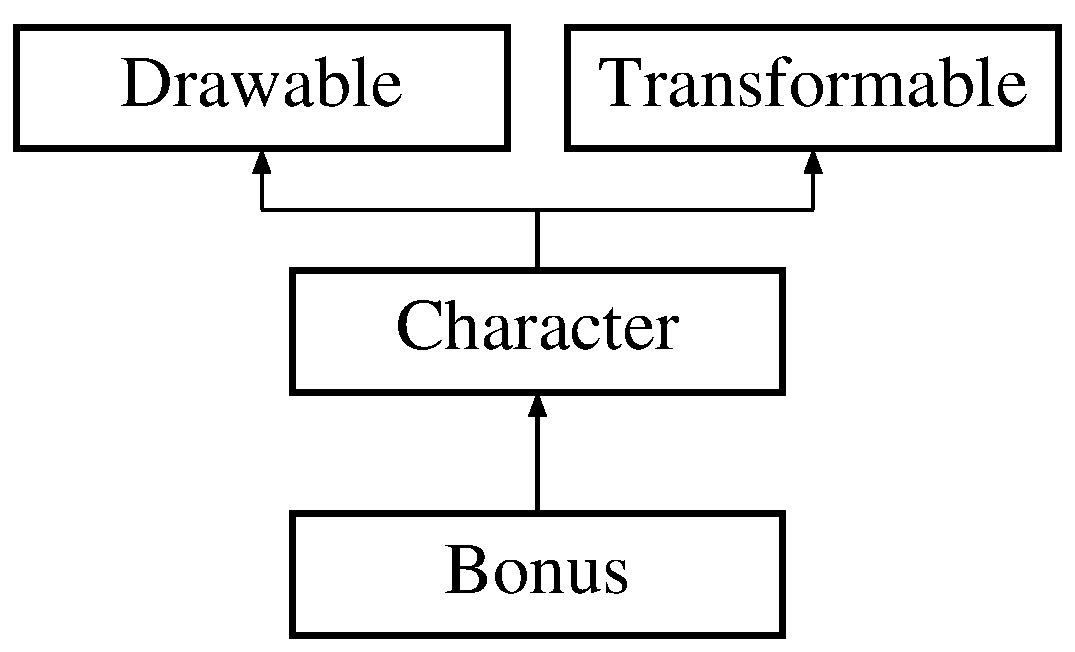
\includegraphics[height=3.000000cm]{class_bonus}
\end{center}
\end{figure}
\subsection*{Public Types}
\begin{DoxyCompactItemize}
\item 
enum \hyperlink{class_bonus_a4325b797efccdaec4e373ceabbfc997f}{Fruit} \{ \hyperlink{class_bonus_a4325b797efccdaec4e373ceabbfc997fa8bce8befd77d72990f2f3f29b949e5aa}{Cherry}, 
\hyperlink{class_bonus_a4325b797efccdaec4e373ceabbfc997fa45dcc835f1401a33b977acb3d2a328cb}{Apple}, 
\hyperlink{class_bonus_a4325b797efccdaec4e373ceabbfc997fad1fd5f77c455ee8d92a95510e32d83fc}{Banana}
 \}
\end{DoxyCompactItemize}
\subsection*{Public Member Functions}
\begin{DoxyCompactItemize}
\item 
\hyperlink{class_bonus_a46346c2f358e8671fc3d4a3c7fae87de}{Bonus} (sf\+::\+Texture \&a\+\_\+\+Texture)
\item 
void \hyperlink{class_bonus_ad6b1650c30b01857ef003a6e9ebf4265}{set\+Fruit} (\hyperlink{class_bonus_a4325b797efccdaec4e373ceabbfc997f}{Fruit} a\+\_\+fruit)
\end{DoxyCompactItemize}
\subsection*{Additional Inherited Members}


\subsection{Detailed Description}
\hyperlink{class_bonus}{Bonus} Class This class inherits from the \hyperlink{class_character}{Character} Class. It renders the fruit bonuses depending on what stage and map the game is currently on. 

Definition at line 21 of file bonus.\+hpp.



\subsection{Member Enumeration Documentation}
\mbox{\Hypertarget{class_bonus_a4325b797efccdaec4e373ceabbfc997f}\label{class_bonus_a4325b797efccdaec4e373ceabbfc997f}} 
\index{Bonus@{Bonus}!Fruit@{Fruit}}
\index{Fruit@{Fruit}!Bonus@{Bonus}}
\subsubsection{\texorpdfstring{Fruit}{Fruit}}
{\footnotesize\ttfamily enum \hyperlink{class_bonus_a4325b797efccdaec4e373ceabbfc997f}{Bonus\+::\+Fruit}}

An enum type Type of fruits that can be rendered \begin{DoxyEnumFields}{Enumerator}
\raisebox{\heightof{T}}[0pt][0pt]{\index{Cherry@{Cherry}!Bonus@{Bonus}}\index{Bonus@{Bonus}!Cherry@{Cherry}}}\mbox{\Hypertarget{class_bonus_a4325b797efccdaec4e373ceabbfc997fa8bce8befd77d72990f2f3f29b949e5aa}\label{class_bonus_a4325b797efccdaec4e373ceabbfc997fa8bce8befd77d72990f2f3f29b949e5aa}} 
Cherry&\\
\hline

\raisebox{\heightof{T}}[0pt][0pt]{\index{Apple@{Apple}!Bonus@{Bonus}}\index{Bonus@{Bonus}!Apple@{Apple}}}\mbox{\Hypertarget{class_bonus_a4325b797efccdaec4e373ceabbfc997fa45dcc835f1401a33b977acb3d2a328cb}\label{class_bonus_a4325b797efccdaec4e373ceabbfc997fa45dcc835f1401a33b977acb3d2a328cb}} 
Apple&\\
\hline

\raisebox{\heightof{T}}[0pt][0pt]{\index{Banana@{Banana}!Bonus@{Bonus}}\index{Bonus@{Bonus}!Banana@{Banana}}}\mbox{\Hypertarget{class_bonus_a4325b797efccdaec4e373ceabbfc997fad1fd5f77c455ee8d92a95510e32d83fc}\label{class_bonus_a4325b797efccdaec4e373ceabbfc997fad1fd5f77c455ee8d92a95510e32d83fc}} 
Banana&\\
\hline

\end{DoxyEnumFields}


Definition at line 28 of file bonus.\+hpp.



\subsection{Constructor \& Destructor Documentation}
\mbox{\Hypertarget{class_bonus_a46346c2f358e8671fc3d4a3c7fae87de}\label{class_bonus_a46346c2f358e8671fc3d4a3c7fae87de}} 
\index{Bonus@{Bonus}!Bonus@{Bonus}}
\index{Bonus@{Bonus}!Bonus@{Bonus}}
\subsubsection{\texorpdfstring{Bonus()}{Bonus()}}
{\footnotesize\ttfamily Bonus\+::\+Bonus (\begin{DoxyParamCaption}\item[{sf\+::\+Texture \&}]{a\+\_\+\+Texture }\end{DoxyParamCaption})}

A \hyperlink{class_bonus}{Bonus} Constructor Initates m\+\_\+visual variable Also sets the default fruit as Apple 

Definition at line 11 of file bonus.\+cpp.



\subsection{Member Function Documentation}
\mbox{\Hypertarget{class_bonus_ad6b1650c30b01857ef003a6e9ebf4265}\label{class_bonus_ad6b1650c30b01857ef003a6e9ebf4265}} 
\index{Bonus@{Bonus}!set\+Fruit@{set\+Fruit}}
\index{set\+Fruit@{set\+Fruit}!Bonus@{Bonus}}
\subsubsection{\texorpdfstring{set\+Fruit()}{setFruit()}}
{\footnotesize\ttfamily void Bonus\+::set\+Fruit (\begin{DoxyParamCaption}\item[{\hyperlink{class_bonus_a4325b797efccdaec4e373ceabbfc997f}{Fruit}}]{a\+\_\+fruit }\end{DoxyParamCaption})}

This function sets what fruit to be rendered on the screen


\begin{DoxyParams}{Parameters}
{\em a\+\_\+fruit} & the fruit instance to be set on screen \\
\hline
\end{DoxyParams}


Definition at line 18 of file bonus.\+cpp.



The documentation for this class was generated from the following files\+:\begin{DoxyCompactItemize}
\item 
smfl\+Test/\hyperlink{bonus_8hpp}{bonus.\+hpp}\item 
smfl\+Test/\hyperlink{bonus_8cpp}{bonus.\+cpp}\end{DoxyCompactItemize}

\hypertarget{class_character}{}\section{Character Class Reference}
\label{class_character}\index{Character@{Character}}


{\ttfamily \#include $<$character.\+hpp$>$}

Inheritance diagram for Character\+:\begin{figure}[H]
\begin{center}
\leavevmode
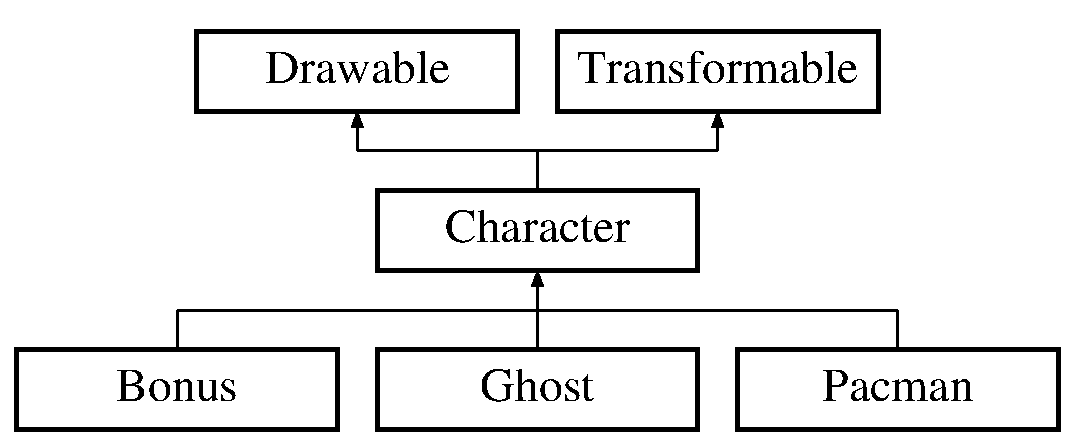
\includegraphics[height=3.000000cm]{class_character}
\end{center}
\end{figure}
\subsection*{Public Member Functions}
\begin{DoxyCompactItemize}
\item 
\hyperlink{class_character_adc27bdd255876169bad2ed0bae0cffb5}{Character} ()
\item 
virtual void \hyperlink{class_character_a89b72b507971ba8648909980d045ed06}{update} (sf\+::\+Time a\+\_\+delta)
\item 
void \hyperlink{class_character_a4af2fa47e778a3d8d6be65d728bed4e8}{set\+Direction} (sf\+::\+Vector2i a\+\_\+direction)
\item 
sf\+::\+Vector2i \hyperlink{class_character_ae8147e847ec305534ef4f2652f3541de}{get\+Direction} () const
\item 
void \hyperlink{class_character_a4a925db15b8f68d2c8d3201ce41f5863}{set\+Maze} (\hyperlink{class_maze}{Maze} $\ast$a\+\_\+maze)
\item 
void \hyperlink{class_character_a37068c523c733698c7f7ad587ccc66a0}{set\+Speed} (float a\+\_\+speed)
\item 
float \hyperlink{class_character_afb7791a8c122e8b88244f0a1a54506c0}{get\+Speed} () const
\item 
bool \hyperlink{class_character_a53d02c2b1c914990e51e0fb84913d151}{will\+Move} () const
\item 
sf\+::\+Float\+Rect \hyperlink{class_character_ab267ab6083ac0b311fc86754ceaed269}{get\+Collision} () const
\end{DoxyCompactItemize}
\subsection*{Protected Member Functions}
\begin{DoxyCompactItemize}
\item 
virtual void \hyperlink{class_character_ab4c0dc6f72c78607b921cf312e10ed35}{change\+Direction} ()
\end{DoxyCompactItemize}


\subsection{Detailed Description}
\hyperlink{class_character}{Character} Class Parent Class to \hyperlink{class_pacman}{Pacman} and \hyperlink{class_ghost}{Ghost}. Inherits from sf\+::\+Drawable and sf\+::\+Transformable. sf\+::\+Transformable can be used as a base class. It is often combined with sf\+::\+Drawable – that\textquotesingle{}s what S\+F\+ML\textquotesingle{}s sprites, texts and shapes do. This is where most of the \hyperlink{class_character}{Character} to \hyperlink{class_maze}{Maze} interaction is happening. Wall Collision, Tunnels, \hyperlink{class_character}{Character} Speed, and Movement Direction are handled in this Class \begin{DoxySeeAlso}{See also}
sf\+::\+Transformable\+: \href{https://www.sfml-dev.org/documentation/2.4.2/classsf_1_1Transformable.php}{\tt https\+://www.\+sfml-\/dev.\+org/documentation/2.\+4.\+2/classsf\+\_\+1\+\_\+1\+Transformable.\+php} 

sf\+::\+Drawable\+: \href{https://www.sfml-dev.org/documentation/2.4.2/classsf_1_1Drawable.php}{\tt https\+://www.\+sfml-\/dev.\+org/documentation/2.\+4.\+2/classsf\+\_\+1\+\_\+1\+Drawable.\+php} 
\end{DoxySeeAlso}


Definition at line 22 of file character.\+hpp.



\subsection{Constructor \& Destructor Documentation}
\mbox{\Hypertarget{class_character_adc27bdd255876169bad2ed0bae0cffb5}\label{class_character_adc27bdd255876169bad2ed0bae0cffb5}} 
\index{Character@{Character}!Character@{Character}}
\index{Character@{Character}!Character@{Character}}
\subsubsection{\texorpdfstring{Character()}{Character()}}
{\footnotesize\ttfamily Character\+::\+Character (\begin{DoxyParamCaption}{ }\end{DoxyParamCaption})}

A \hyperlink{class_character}{Character} Constructor Initiates the following member variables
\begin{DoxyItemize}
\item m\+\_\+maze
\item m\+\_\+speed
\item m\+\_\+current\+Direction
\item m\+\_\+next\+Direction
\item m\+\_\+prev\+Intersecion 
\end{DoxyItemize}

Definition at line 15 of file character.\+cpp.



\subsection{Member Function Documentation}
\mbox{\Hypertarget{class_character_ab4c0dc6f72c78607b921cf312e10ed35}\label{class_character_ab4c0dc6f72c78607b921cf312e10ed35}} 
\index{Character@{Character}!change\+Direction@{change\+Direction}}
\index{change\+Direction@{change\+Direction}!Character@{Character}}
\subsubsection{\texorpdfstring{change\+Direction()}{changeDirection()}}
{\footnotesize\ttfamily virtual void Character\+::change\+Direction (\begin{DoxyParamCaption}{ }\end{DoxyParamCaption})\hspace{0.3cm}{\ttfamily [inline]}, {\ttfamily [protected]}, {\ttfamily [virtual]}}

This is a virtual function that the ghost class uses for it\textquotesingle{}s pathfinding AI

\begin{DoxySeeAlso}{See also}
\hyperlink{class_ghost}{Ghost} Class 
\end{DoxySeeAlso}


Reimplemented in \hyperlink{class_ghost_a08831fa01afa61f91365ce82cf33bf1b}{Ghost}.



Definition at line 101 of file character.\+hpp.

\mbox{\Hypertarget{class_character_ab267ab6083ac0b311fc86754ceaed269}\label{class_character_ab267ab6083ac0b311fc86754ceaed269}} 
\index{Character@{Character}!get\+Collision@{get\+Collision}}
\index{get\+Collision@{get\+Collision}!Character@{Character}}
\subsubsection{\texorpdfstring{get\+Collision()}{getCollision()}}
{\footnotesize\ttfamily sf\+::\+Float\+Rect Character\+::get\+Collision (\begin{DoxyParamCaption}{ }\end{DoxyParamCaption}) const}

This function creates a rectangle bound around the character sprite which helps detect collision

\begin{DoxyReturn}{Returns}
Returns the position/rotation/scale/origin of the collision box 
\end{DoxyReturn}


Definition at line 38 of file character.\+cpp.

\mbox{\Hypertarget{class_character_ae8147e847ec305534ef4f2652f3541de}\label{class_character_ae8147e847ec305534ef4f2652f3541de}} 
\index{Character@{Character}!get\+Direction@{get\+Direction}}
\index{get\+Direction@{get\+Direction}!Character@{Character}}
\subsubsection{\texorpdfstring{get\+Direction()}{getDirection()}}
{\footnotesize\ttfamily sf\+::\+Vector2i Character\+::get\+Direction (\begin{DoxyParamCaption}{ }\end{DoxyParamCaption}) const}

This function is a get function for the m\+\_\+current\+Direction which is a private variable

\begin{DoxyReturn}{Returns}
Returns the direction that the character is taking in the map 
\end{DoxyReturn}


Definition at line 30 of file character.\+cpp.

\mbox{\Hypertarget{class_character_afb7791a8c122e8b88244f0a1a54506c0}\label{class_character_afb7791a8c122e8b88244f0a1a54506c0}} 
\index{Character@{Character}!get\+Speed@{get\+Speed}}
\index{get\+Speed@{get\+Speed}!Character@{Character}}
\subsubsection{\texorpdfstring{get\+Speed()}{getSpeed()}}
{\footnotesize\ttfamily float Character\+::get\+Speed (\begin{DoxyParamCaption}{ }\end{DoxyParamCaption}) const}

This function is a get function for the m\+\_\+speed which is a private variable

\begin{DoxyReturn}{Returns}
Returns the character\textquotesingle{}s movement speed 
\end{DoxyReturn}


Definition at line 138 of file character.\+cpp.

\mbox{\Hypertarget{class_character_a4af2fa47e778a3d8d6be65d728bed4e8}\label{class_character_a4af2fa47e778a3d8d6be65d728bed4e8}} 
\index{Character@{Character}!set\+Direction@{set\+Direction}}
\index{set\+Direction@{set\+Direction}!Character@{Character}}
\subsubsection{\texorpdfstring{set\+Direction()}{setDirection()}}
{\footnotesize\ttfamily void Character\+::set\+Direction (\begin{DoxyParamCaption}\item[{sf\+::\+Vector2i}]{a\+\_\+direction }\end{DoxyParamCaption})}

This function takes a sfml integer vector as a position and sets which direction the character needs to go. This function also processes all interaction that the character has with the map such ass Wall Collision, and the Tunnel. It also controls the \hyperlink{class_ghost}{Ghost}\textquotesingle{}s movements


\begin{DoxyParams}{Parameters}
{\em a\+\_\+direction} & the direction the character is heading \\
\hline
\end{DoxyParams}


Definition at line 27 of file character.\+cpp.

\mbox{\Hypertarget{class_character_a4a925db15b8f68d2c8d3201ce41f5863}\label{class_character_a4a925db15b8f68d2c8d3201ce41f5863}} 
\index{Character@{Character}!set\+Maze@{set\+Maze}}
\index{set\+Maze@{set\+Maze}!Character@{Character}}
\subsubsection{\texorpdfstring{set\+Maze()}{setMaze()}}
{\footnotesize\ttfamily void Character\+::set\+Maze (\begin{DoxyParamCaption}\item[{\hyperlink{class_maze}{Maze} $\ast$}]{a\+\_\+maze }\end{DoxyParamCaption})}

This function assigns the current game instance to the character class


\begin{DoxyParams}{Parameters}
{\em a\+\_\+maze} & the maze instance \\
\hline
\end{DoxyParams}


Definition at line 23 of file character.\+cpp.

\mbox{\Hypertarget{class_character_a37068c523c733698c7f7ad587ccc66a0}\label{class_character_a37068c523c733698c7f7ad587ccc66a0}} 
\index{Character@{Character}!set\+Speed@{set\+Speed}}
\index{set\+Speed@{set\+Speed}!Character@{Character}}
\subsubsection{\texorpdfstring{set\+Speed()}{setSpeed()}}
{\footnotesize\ttfamily void Character\+::set\+Speed (\begin{DoxyParamCaption}\item[{float}]{a\+\_\+speed }\end{DoxyParamCaption})}

This function registers how fast the character moves around the map


\begin{DoxyParams}{Parameters}
{\em a\+\_\+speed} & the character\textquotesingle{}s movement speed \\
\hline
\end{DoxyParams}


Definition at line 134 of file character.\+cpp.

\mbox{\Hypertarget{class_character_a89b72b507971ba8648909980d045ed06}\label{class_character_a89b72b507971ba8648909980d045ed06}} 
\index{Character@{Character}!update@{update}}
\index{update@{update}!Character@{Character}}
\subsubsection{\texorpdfstring{update()}{update()}}
{\footnotesize\ttfamily void Character\+::update (\begin{DoxyParamCaption}\item[{sf\+::\+Time}]{a\+\_\+delta }\end{DoxyParamCaption})\hspace{0.3cm}{\ttfamily [virtual]}}

A virtual function


\begin{DoxyParams}{Parameters}
{\em a\+\_\+delta} & the current time \\
\hline
\end{DoxyParams}
\begin{DoxySeeAlso}{See also}
\hyperlink{class_pacman}{Pacman} Class 

\hyperlink{class_ghost}{Ghost} Class 
\end{DoxySeeAlso}


Reimplemented in \hyperlink{class_ghost_a164e0607f7ea0d72d756bdf964e66b90}{Ghost}, and \hyperlink{class_pacman_a6badb47a28223991a1eb540f9d970e77}{Pacman}.



Definition at line 43 of file character.\+cpp.

\mbox{\Hypertarget{class_character_a53d02c2b1c914990e51e0fb84913d151}\label{class_character_a53d02c2b1c914990e51e0fb84913d151}} 
\index{Character@{Character}!will\+Move@{will\+Move}}
\index{will\+Move@{will\+Move}!Character@{Character}}
\subsubsection{\texorpdfstring{will\+Move()}{willMove()}}
{\footnotesize\ttfamily bool Character\+::will\+Move (\begin{DoxyParamCaption}{ }\end{DoxyParamCaption}) const}

This function checks wheter the next direction is a valid position that the character can go to

\begin{DoxyReturn}{Returns}
Returns true if the next direction not a wall 
\end{DoxyReturn}


Definition at line 34 of file character.\+cpp.



The documentation for this class was generated from the following files\+:\begin{DoxyCompactItemize}
\item 
smfl\+Test/\hyperlink{character_8hpp}{character.\+hpp}\item 
smfl\+Test/\hyperlink{character_8cpp}{character.\+cpp}\end{DoxyCompactItemize}

\hypertarget{class_game}{}\section{Game Class Reference}
\label{class_game}\index{Game@{Game}}


{\ttfamily \#include $<$game.\+hpp$>$}

\subsection*{Public Member Functions}
\begin{DoxyCompactItemize}
\item 
\hyperlink{class_game_ad59df6562a58a614fda24622d3715b65}{Game} ()
\item 
\hyperlink{class_game_ae3d112ca6e0e55150d2fdbc704474530}{$\sim$\+Game} ()
\item 
void \hyperlink{class_game_a1ab78f5ed0d5ea879157357cf2fb2afa}{run} ()
\item 
sf\+::\+Font \& \hyperlink{class_game_a813ff20fa498389e4bb120090803676b}{get\+Font} ()
\item 
sf\+::\+Texture \& \hyperlink{class_game_a4eb607b287a0aa0238339454399edc8b}{get\+Logo} ()
\item 
sf\+::\+Texture \& \hyperlink{class_game_aa231abe1d7a36b55599ca459c815b2a5}{get\+Texture} ()
\item 
void \hyperlink{class_game_aead31c173174cd4251542403a9e1e111}{change\+Game\+State} (\hyperlink{class_game_state_a81618e0403319d48e9f25347111f8157}{Game\+State\+::\+State} a\+\_\+game\+State)
\end{DoxyCompactItemize}


\subsection{Detailed Description}
\hyperlink{class_game}{Game} Class This Class is the center of the whole game. The game states are intiated and runs through this class. The game assets are also loaded from here. 

Definition at line 23 of file game.\+hpp.



\subsection{Constructor \& Destructor Documentation}
\mbox{\Hypertarget{class_game_ad59df6562a58a614fda24622d3715b65}\label{class_game_ad59df6562a58a614fda24622d3715b65}} 
\index{Game@{Game}!Game@{Game}}
\index{Game@{Game}!Game@{Game}}
\subsubsection{\texorpdfstring{Game()}{Game()}}
{\footnotesize\ttfamily Game\+::\+Game (\begin{DoxyParamCaption}{ }\end{DoxyParamCaption})}

A \hyperlink{class_game}{Game} Constuctor Initates m\+\_\+window variable to a 448 x 528 pixel screen Also loads up game assets and sets up all the game states. 

Definition at line 17 of file game.\+cpp.

\mbox{\Hypertarget{class_game_ae3d112ca6e0e55150d2fdbc704474530}\label{class_game_ae3d112ca6e0e55150d2fdbc704474530}} 
\index{Game@{Game}!````~Game@{$\sim$\+Game}}
\index{````~Game@{$\sim$\+Game}!Game@{Game}}
\subsubsection{\texorpdfstring{$\sim$\+Game()}{~Game()}}
{\footnotesize\ttfamily Game\+::$\sim$\+Game (\begin{DoxyParamCaption}{ }\end{DoxyParamCaption})}

A \hyperlink{class_game}{Game} Destructor 

Definition at line 40 of file game.\+cpp.



\subsection{Member Function Documentation}
\mbox{\Hypertarget{class_game_aead31c173174cd4251542403a9e1e111}\label{class_game_aead31c173174cd4251542403a9e1e111}} 
\index{Game@{Game}!change\+Game\+State@{change\+Game\+State}}
\index{change\+Game\+State@{change\+Game\+State}!Game@{Game}}
\subsubsection{\texorpdfstring{change\+Game\+State()}{changeGameState()}}
{\footnotesize\ttfamily void Game\+::change\+Game\+State (\begin{DoxyParamCaption}\item[{\hyperlink{class_game_state_a81618e0403319d48e9f25347111f8157}{Game\+State\+::\+State}}]{a\+\_\+game\+State }\end{DoxyParamCaption})}

This function changes the current game state


\begin{DoxyParams}{Parameters}
{\em a\+\_\+game\+State} & the gamestate to replace the current one \\
\hline
\end{DoxyParams}


Definition at line 92 of file game.\+cpp.

\mbox{\Hypertarget{class_game_a813ff20fa498389e4bb120090803676b}\label{class_game_a813ff20fa498389e4bb120090803676b}} 
\index{Game@{Game}!get\+Font@{get\+Font}}
\index{get\+Font@{get\+Font}!Game@{Game}}
\subsubsection{\texorpdfstring{get\+Font()}{getFont()}}
{\footnotesize\ttfamily sf\+::\+Font \& Game\+::get\+Font (\begin{DoxyParamCaption}{ }\end{DoxyParamCaption})}

This is a get function for m\+\_\+game\+Font

\begin{DoxyReturn}{Returns}
returns the game font that was loaded 
\end{DoxyReturn}


Definition at line 97 of file game.\+cpp.

\mbox{\Hypertarget{class_game_a4eb607b287a0aa0238339454399edc8b}\label{class_game_a4eb607b287a0aa0238339454399edc8b}} 
\index{Game@{Game}!get\+Logo@{get\+Logo}}
\index{get\+Logo@{get\+Logo}!Game@{Game}}
\subsubsection{\texorpdfstring{get\+Logo()}{getLogo()}}
{\footnotesize\ttfamily sf\+::\+Texture \& Game\+::get\+Logo (\begin{DoxyParamCaption}{ }\end{DoxyParamCaption})}

This is a get function for m\+\_\+game\+Logo

\begin{DoxyReturn}{Returns}
returns the game logo that was loaded 
\end{DoxyReturn}


Definition at line 101 of file game.\+cpp.

\mbox{\Hypertarget{class_game_aa231abe1d7a36b55599ca459c815b2a5}\label{class_game_aa231abe1d7a36b55599ca459c815b2a5}} 
\index{Game@{Game}!get\+Texture@{get\+Texture}}
\index{get\+Texture@{get\+Texture}!Game@{Game}}
\subsubsection{\texorpdfstring{get\+Texture()}{getTexture()}}
{\footnotesize\ttfamily sf\+::\+Texture \& Game\+::get\+Texture (\begin{DoxyParamCaption}{ }\end{DoxyParamCaption})}

This is a get function for m\+\_\+game\+Texture

\begin{DoxyReturn}{Returns}
returns the game sprite sheet that was loaded 
\end{DoxyReturn}


Definition at line 105 of file game.\+cpp.

\mbox{\Hypertarget{class_game_a1ab78f5ed0d5ea879157357cf2fb2afa}\label{class_game_a1ab78f5ed0d5ea879157357cf2fb2afa}} 
\index{Game@{Game}!run@{run}}
\index{run@{run}!Game@{Game}}
\subsubsection{\texorpdfstring{run()}{run()}}
{\footnotesize\ttfamily void Game\+::run (\begin{DoxyParamCaption}{ }\end{DoxyParamCaption})}

This function fires up the game. \hyperlink{class_game}{Game} time, Key Inputs and window rendering all run through this function 

Definition at line 46 of file game.\+cpp.



The documentation for this class was generated from the following files\+:\begin{DoxyCompactItemize}
\item 
smfl\+Test/\hyperlink{game_8hpp}{game.\+hpp}\item 
smfl\+Test/\hyperlink{game_8cpp}{game.\+cpp}\end{DoxyCompactItemize}

\hypertarget{class_game_state}{}\section{Game\+State Class Reference}
\label{class_game_state}\index{Game\+State@{Game\+State}}


{\ttfamily \#include $<$game\+State.\+hpp$>$}

Inheritance diagram for Game\+State\+:\begin{figure}[H]
\begin{center}
\leavevmode
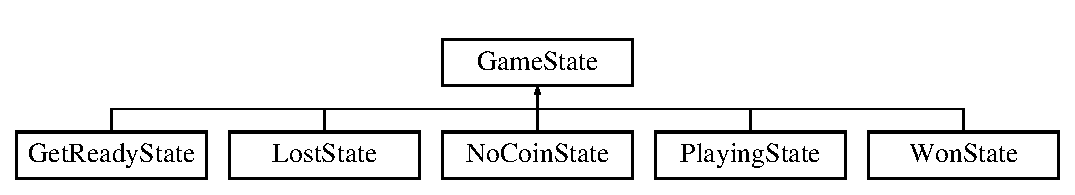
\includegraphics[height=2.000000cm]{class_game_state}
\end{center}
\end{figure}
\subsection*{Public Types}
\begin{DoxyCompactItemize}
\item 
enum \hyperlink{class_game_state_a81618e0403319d48e9f25347111f8157}{State} \{ \newline
\hyperlink{class_game_state_a81618e0403319d48e9f25347111f8157ad554378cedc28c806c2abc5da3091455}{no\+Coin}, 
\hyperlink{class_game_state_a81618e0403319d48e9f25347111f8157a1b334dd547fee485fccb33f336e64922}{get\+Ready}, 
\hyperlink{class_game_state_a81618e0403319d48e9f25347111f8157a0c7c919903ffb50f3d56b0ef11fb5532}{Playing}, 
\hyperlink{class_game_state_a81618e0403319d48e9f25347111f8157aec55aaf1858ada4e8896fcad78f574a8}{Won}, 
\newline
\hyperlink{class_game_state_a81618e0403319d48e9f25347111f8157a4f2379bcd5431f1a2fd56f96c9b8ebfb}{Lost}, 
\hyperlink{class_game_state_a81618e0403319d48e9f25347111f8157a9d9e2cb82e9bb0c70fa650a2642c5271}{Count}
 \}
\end{DoxyCompactItemize}
\subsection*{Public Member Functions}
\begin{DoxyCompactItemize}
\item 
\hyperlink{class_game_state_a294ebc243ce5cf5f845b8548aba8e723}{Game\+State} (\hyperlink{class_game}{Game} $\ast$a\+\_\+game)
\item 
\hyperlink{class_game}{Game} $\ast$ \hyperlink{class_game_state_a7f1afbce585f48311006ddb00c26e32f}{get\+Game} () const
\item 
virtual void \hyperlink{class_game_state_a4cd6f5b4ad23fc08dca287df26d94b94}{insert\+Coin} ()=0
\item 
virtual void \hyperlink{class_game_state_aa14eeaf244bcf19b7013af75cb722dde}{press\+Button} ()=0
\item 
virtual void \hyperlink{class_game_state_aaae8c1b3ae6969eb2dd81bfc12fbf43f}{move\+Stick} (sf\+::\+Vector2i a\+\_\+direction)=0
\item 
virtual void \hyperlink{class_game_state_ab1fe4312f7ce88e7dc11f9935dee67d1}{update} (sf\+::\+Time delta)=0
\item 
virtual void \hyperlink{class_game_state_a5ffd5ce9acb7499ddef613e8836d1ef8}{draw} (sf\+::\+Render\+Window \&a\+\_\+window)=0
\end{DoxyCompactItemize}


\subsection{Detailed Description}
\hyperlink{class_game_state}{Game\+State} Class Parent class to \hyperlink{class_no_coin_state}{No\+Coin\+State}, \hyperlink{class_get_ready_state}{Get\+Ready\+State}, \hyperlink{class_lost_state}{Lost\+State}, \hyperlink{class_won_state}{Won\+State}, and Playing State. This is where the \hyperlink{class_game_state}{Game\+State} loops circulates. Every \hyperlink{class_game_state}{Game\+State} renders its own window and calls the next appropriate game state. This is also know as a Finite State Machine Pattern. 

Definition at line 25 of file game\+State.\+hpp.



\subsection{Member Enumeration Documentation}
\mbox{\Hypertarget{class_game_state_a81618e0403319d48e9f25347111f8157}\label{class_game_state_a81618e0403319d48e9f25347111f8157}} 
\index{Game\+State@{Game\+State}!State@{State}}
\index{State@{State}!Game\+State@{Game\+State}}
\subsubsection{\texorpdfstring{State}{State}}
{\footnotesize\ttfamily enum \hyperlink{class_game_state_a81618e0403319d48e9f25347111f8157}{Game\+State\+::\+State}}

An enum type The different game states \begin{DoxyEnumFields}{Enumerator}
\raisebox{\heightof{T}}[0pt][0pt]{\index{no\+Coin@{no\+Coin}!Game\+State@{Game\+State}}\index{Game\+State@{Game\+State}!no\+Coin@{no\+Coin}}}\mbox{\Hypertarget{class_game_state_a81618e0403319d48e9f25347111f8157ad554378cedc28c806c2abc5da3091455}\label{class_game_state_a81618e0403319d48e9f25347111f8157ad554378cedc28c806c2abc5da3091455}} 
no\+Coin&\\
\hline

\raisebox{\heightof{T}}[0pt][0pt]{\index{get\+Ready@{get\+Ready}!Game\+State@{Game\+State}}\index{Game\+State@{Game\+State}!get\+Ready@{get\+Ready}}}\mbox{\Hypertarget{class_game_state_a81618e0403319d48e9f25347111f8157a1b334dd547fee485fccb33f336e64922}\label{class_game_state_a81618e0403319d48e9f25347111f8157a1b334dd547fee485fccb33f336e64922}} 
get\+Ready&\\
\hline

\raisebox{\heightof{T}}[0pt][0pt]{\index{Playing@{Playing}!Game\+State@{Game\+State}}\index{Game\+State@{Game\+State}!Playing@{Playing}}}\mbox{\Hypertarget{class_game_state_a81618e0403319d48e9f25347111f8157a0c7c919903ffb50f3d56b0ef11fb5532}\label{class_game_state_a81618e0403319d48e9f25347111f8157a0c7c919903ffb50f3d56b0ef11fb5532}} 
Playing&\\
\hline

\raisebox{\heightof{T}}[0pt][0pt]{\index{Won@{Won}!Game\+State@{Game\+State}}\index{Game\+State@{Game\+State}!Won@{Won}}}\mbox{\Hypertarget{class_game_state_a81618e0403319d48e9f25347111f8157aec55aaf1858ada4e8896fcad78f574a8}\label{class_game_state_a81618e0403319d48e9f25347111f8157aec55aaf1858ada4e8896fcad78f574a8}} 
Won&\\
\hline

\raisebox{\heightof{T}}[0pt][0pt]{\index{Lost@{Lost}!Game\+State@{Game\+State}}\index{Game\+State@{Game\+State}!Lost@{Lost}}}\mbox{\Hypertarget{class_game_state_a81618e0403319d48e9f25347111f8157a4f2379bcd5431f1a2fd56f96c9b8ebfb}\label{class_game_state_a81618e0403319d48e9f25347111f8157a4f2379bcd5431f1a2fd56f96c9b8ebfb}} 
Lost&\\
\hline

\raisebox{\heightof{T}}[0pt][0pt]{\index{Count@{Count}!Game\+State@{Game\+State}}\index{Game\+State@{Game\+State}!Count@{Count}}}\mbox{\Hypertarget{class_game_state_a81618e0403319d48e9f25347111f8157a9d9e2cb82e9bb0c70fa650a2642c5271}\label{class_game_state_a81618e0403319d48e9f25347111f8157a9d9e2cb82e9bb0c70fa650a2642c5271}} 
Count&\\
\hline

\end{DoxyEnumFields}


Definition at line 31 of file game\+State.\+hpp.



\subsection{Constructor \& Destructor Documentation}
\mbox{\Hypertarget{class_game_state_a294ebc243ce5cf5f845b8548aba8e723}\label{class_game_state_a294ebc243ce5cf5f845b8548aba8e723}} 
\index{Game\+State@{Game\+State}!Game\+State@{Game\+State}}
\index{Game\+State@{Game\+State}!Game\+State@{Game\+State}}
\subsubsection{\texorpdfstring{Game\+State()}{GameState()}}
{\footnotesize\ttfamily Game\+State\+::\+Game\+State (\begin{DoxyParamCaption}\item[{\hyperlink{class_game}{Game} $\ast$}]{a\+\_\+game }\end{DoxyParamCaption})}

A \hyperlink{class_game_state}{Game\+State} Constructor Initiates an instance of the game, and the same game instance will be used for the five different game states 
\begin{DoxyParams}{Parameters}
{\em a\+\_\+game} & the current game instance \\
\hline
\end{DoxyParams}


Definition at line 22 of file game\+State.\+cpp.



\subsection{Member Function Documentation}
\mbox{\Hypertarget{class_game_state_a5ffd5ce9acb7499ddef613e8836d1ef8}\label{class_game_state_a5ffd5ce9acb7499ddef613e8836d1ef8}} 
\index{Game\+State@{Game\+State}!draw@{draw}}
\index{draw@{draw}!Game\+State@{Game\+State}}
\subsubsection{\texorpdfstring{draw()}{draw()}}
{\footnotesize\ttfamily virtual void Game\+State\+::draw (\begin{DoxyParamCaption}\item[{sf\+::\+Render\+Window \&}]{a\+\_\+window }\end{DoxyParamCaption})\hspace{0.3cm}{\ttfamily [pure virtual]}}

A pure virtual function


\begin{DoxyParams}{Parameters}
{\em a\+\_\+window} & the window where the game is rendered \\
\hline
\end{DoxyParams}


Implemented in \hyperlink{class_lost_state_acfdefa77d7ed756a1052d39ed2de8786}{Lost\+State}, \hyperlink{class_won_state_a88bcef07ae234fe7ba672d1c6628d2c0}{Won\+State}, \hyperlink{class_playing_state_aa6c7033a5c734ba1ae4aae0905554d61}{Playing\+State}, \hyperlink{class_get_ready_state_a5526ece0f8f8becab78b78fbc7919045}{Get\+Ready\+State}, and \hyperlink{class_no_coin_state_ab1e920e22b90f9d36954e75ea49c3f9b}{No\+Coin\+State}.

\mbox{\Hypertarget{class_game_state_a7f1afbce585f48311006ddb00c26e32f}\label{class_game_state_a7f1afbce585f48311006ddb00c26e32f}} 
\index{Game\+State@{Game\+State}!get\+Game@{get\+Game}}
\index{get\+Game@{get\+Game}!Game\+State@{Game\+State}}
\subsubsection{\texorpdfstring{get\+Game()}{getGame()}}
{\footnotesize\ttfamily \hyperlink{class_game}{Game} $\ast$ Game\+State\+::get\+Game (\begin{DoxyParamCaption}{ }\end{DoxyParamCaption}) const}

This function is a get function for m\+\_\+game

\begin{DoxyReturn}{Returns}
returns the current game instance 
\end{DoxyReturn}


Definition at line 142 of file game\+State.\+cpp.

\mbox{\Hypertarget{class_game_state_a4cd6f5b4ad23fc08dca287df26d94b94}\label{class_game_state_a4cd6f5b4ad23fc08dca287df26d94b94}} 
\index{Game\+State@{Game\+State}!insert\+Coin@{insert\+Coin}}
\index{insert\+Coin@{insert\+Coin}!Game\+State@{Game\+State}}
\subsubsection{\texorpdfstring{insert\+Coin()}{insertCoin()}}
{\footnotesize\ttfamily virtual void Game\+State\+::insert\+Coin (\begin{DoxyParamCaption}{ }\end{DoxyParamCaption})\hspace{0.3cm}{\ttfamily [pure virtual]}}

A pure virtual function 

Implemented in \hyperlink{class_lost_state_aa35179942033d9ab54fbcd7122f40497}{Lost\+State}, \hyperlink{class_won_state_aeaab03fa1a39188c19107047417c65b6}{Won\+State}, \hyperlink{class_playing_state_a936d41a2041ace2ccb67a9b779d113a7}{Playing\+State}, \hyperlink{class_get_ready_state_afac1da927d38cf32960f2370856ec9f6}{Get\+Ready\+State}, and \hyperlink{class_no_coin_state_a417209eadad2f71284cf09d369bc389e}{No\+Coin\+State}.

\mbox{\Hypertarget{class_game_state_aaae8c1b3ae6969eb2dd81bfc12fbf43f}\label{class_game_state_aaae8c1b3ae6969eb2dd81bfc12fbf43f}} 
\index{Game\+State@{Game\+State}!move\+Stick@{move\+Stick}}
\index{move\+Stick@{move\+Stick}!Game\+State@{Game\+State}}
\subsubsection{\texorpdfstring{move\+Stick()}{moveStick()}}
{\footnotesize\ttfamily virtual void Game\+State\+::move\+Stick (\begin{DoxyParamCaption}\item[{sf\+::\+Vector2i}]{a\+\_\+direction }\end{DoxyParamCaption})\hspace{0.3cm}{\ttfamily [pure virtual]}}

A pure virtual function


\begin{DoxyParams}{Parameters}
{\em a\+\_\+direction} & the desired direction \\
\hline
\end{DoxyParams}


Implemented in \hyperlink{class_lost_state_abc978a14604451eee5e0373b4ad374c8}{Lost\+State}, \hyperlink{class_won_state_a56b272d25511e6a302136d308648464b}{Won\+State}, \hyperlink{class_playing_state_af205fbb130a2c83b260d80359de914e8}{Playing\+State}, \hyperlink{class_get_ready_state_a0a7f1548b4c58e8bd5634ceb59ba7b9b}{Get\+Ready\+State}, and \hyperlink{class_no_coin_state_a9fe8f36082705e6f5833244890093adc}{No\+Coin\+State}.

\mbox{\Hypertarget{class_game_state_aa14eeaf244bcf19b7013af75cb722dde}\label{class_game_state_aa14eeaf244bcf19b7013af75cb722dde}} 
\index{Game\+State@{Game\+State}!press\+Button@{press\+Button}}
\index{press\+Button@{press\+Button}!Game\+State@{Game\+State}}
\subsubsection{\texorpdfstring{press\+Button()}{pressButton()}}
{\footnotesize\ttfamily virtual void Game\+State\+::press\+Button (\begin{DoxyParamCaption}{ }\end{DoxyParamCaption})\hspace{0.3cm}{\ttfamily [pure virtual]}}

A pure virtual function 

Implemented in \hyperlink{class_lost_state_ab0ec749961cfe909dc61289d14444a71}{Lost\+State}, \hyperlink{class_won_state_ab17f101d9ab90e60259e28b8775a76ec}{Won\+State}, \hyperlink{class_playing_state_ae59ff244a6cd4a3c6f6fcaef41f4d8c5}{Playing\+State}, \hyperlink{class_get_ready_state_a414a505ec783b1bf577b1b859abaee46}{Get\+Ready\+State}, and \hyperlink{class_no_coin_state_a47dd2924ce9601b45ee11e0d9b8452f7}{No\+Coin\+State}.

\mbox{\Hypertarget{class_game_state_ab1fe4312f7ce88e7dc11f9935dee67d1}\label{class_game_state_ab1fe4312f7ce88e7dc11f9935dee67d1}} 
\index{Game\+State@{Game\+State}!update@{update}}
\index{update@{update}!Game\+State@{Game\+State}}
\subsubsection{\texorpdfstring{update()}{update()}}
{\footnotesize\ttfamily virtual void Game\+State\+::update (\begin{DoxyParamCaption}\item[{sf\+::\+Time}]{delta }\end{DoxyParamCaption})\hspace{0.3cm}{\ttfamily [pure virtual]}}

A pure virtual function


\begin{DoxyParams}{Parameters}
{\em delta} & the current time \\
\hline
\end{DoxyParams}


Implemented in \hyperlink{class_lost_state_a16d5e12284d03f8dd6b25a897b25839b}{Lost\+State}, \hyperlink{class_won_state_a0ea91513e3df2eafbe8ef7b9810eaff1}{Won\+State}, \hyperlink{class_playing_state_a62b3904b8a971fed2f8fab4eb73bd9e5}{Playing\+State}, \hyperlink{class_get_ready_state_a6e5a1035b4ee7a52aa28027a0b99dd8a}{Get\+Ready\+State}, and \hyperlink{class_no_coin_state_af0194851310c6df176770713341a8b80}{No\+Coin\+State}.



The documentation for this class was generated from the following files\+:\begin{DoxyCompactItemize}
\item 
smfl\+Test/\hyperlink{game_state_8hpp}{game\+State.\+hpp}\item 
smfl\+Test/\hyperlink{game_state_8cpp}{game\+State.\+cpp}\end{DoxyCompactItemize}

\hypertarget{class_get_ready_state}{}\section{Get\+Ready\+State Class Reference}
\label{class_get_ready_state}\index{Get\+Ready\+State@{Get\+Ready\+State}}


{\ttfamily \#include $<$game\+State.\+hpp$>$}

Inheritance diagram for Get\+Ready\+State\+:\begin{figure}[H]
\begin{center}
\leavevmode
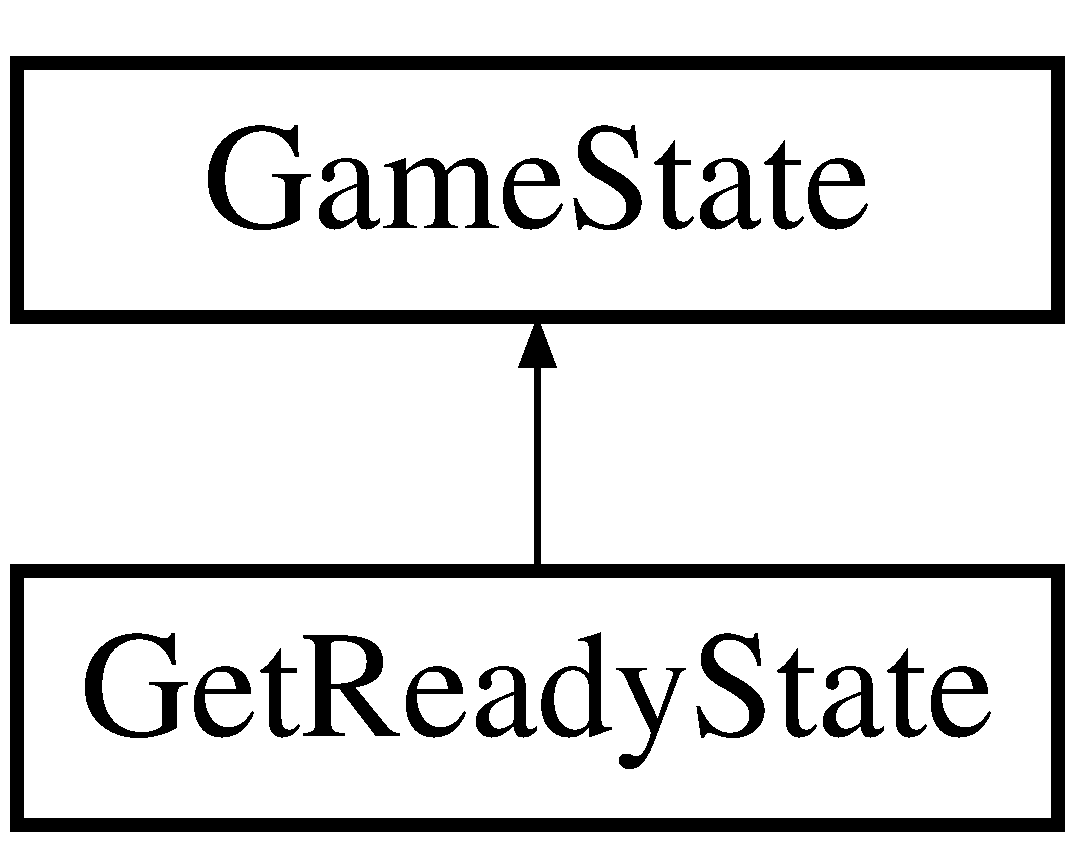
\includegraphics[height=2.000000cm]{class_get_ready_state}
\end{center}
\end{figure}
\subsection*{Public Member Functions}
\begin{DoxyCompactItemize}
\item 
\hyperlink{class_get_ready_state_a227e45622dad03369a88024b54df0e92}{Get\+Ready\+State} (\hyperlink{class_game}{Game} $\ast$a\+\_\+game)
\item 
void \hyperlink{class_get_ready_state_afac1da927d38cf32960f2370856ec9f6}{insert\+Coin} ()
\item 
void \hyperlink{class_get_ready_state_a414a505ec783b1bf577b1b859abaee46}{press\+Button} ()
\item 
void \hyperlink{class_get_ready_state_a0a7f1548b4c58e8bd5634ceb59ba7b9b}{move\+Stick} (sf\+::\+Vector2i a\+\_\+direction)
\item 
void \hyperlink{class_get_ready_state_a6e5a1035b4ee7a52aa28027a0b99dd8a}{update} (sf\+::\+Time a\+\_\+delta)
\item 
void \hyperlink{class_get_ready_state_a5526ece0f8f8becab78b78fbc7919045}{draw} (sf\+::\+Render\+Window \&a\+\_\+window)
\end{DoxyCompactItemize}
\subsection*{Additional Inherited Members}


\subsection{Detailed Description}
\hyperlink{class_get_ready_state}{Get\+Ready\+State} This class inherits from the \hyperlink{class_game_state}{Game\+State} Class. This game state is launched right before the game is played. During the state it waits for an input(\char`\"{}\+S\char`\"{}) to ensure that the player is ready to play. 

Definition at line 165 of file game\+State.\+hpp.



\subsection{Constructor \& Destructor Documentation}
\mbox{\Hypertarget{class_get_ready_state_a227e45622dad03369a88024b54df0e92}\label{class_get_ready_state_a227e45622dad03369a88024b54df0e92}} 
\index{Get\+Ready\+State@{Get\+Ready\+State}!Get\+Ready\+State@{Get\+Ready\+State}}
\index{Get\+Ready\+State@{Get\+Ready\+State}!Get\+Ready\+State@{Get\+Ready\+State}}
\subsubsection{\texorpdfstring{Get\+Ready\+State()}{GetReadyState()}}
{\footnotesize\ttfamily Get\+Ready\+State\+::\+Get\+Ready\+State (\begin{DoxyParamCaption}\item[{\hyperlink{class_game}{Game} $\ast$}]{a\+\_\+game }\end{DoxyParamCaption})}

A \hyperlink{class_get_ready_state}{Get\+Ready\+State} Consturctor Initiates the \char`\"{}\+Press S to Start\char`\"{} text to be rendered to the screen 
\begin{DoxyParams}{Parameters}
{\em a\+\_\+game} & the current game instance \\
\hline
\end{DoxyParams}


Definition at line 41 of file game\+State.\+cpp.



\subsection{Member Function Documentation}
\mbox{\Hypertarget{class_get_ready_state_a5526ece0f8f8becab78b78fbc7919045}\label{class_get_ready_state_a5526ece0f8f8becab78b78fbc7919045}} 
\index{Get\+Ready\+State@{Get\+Ready\+State}!draw@{draw}}
\index{draw@{draw}!Get\+Ready\+State@{Get\+Ready\+State}}
\subsubsection{\texorpdfstring{draw()}{draw()}}
{\footnotesize\ttfamily void Get\+Ready\+State\+::draw (\begin{DoxyParamCaption}\item[{sf\+::\+Render\+Window \&}]{a\+\_\+window }\end{DoxyParamCaption})\hspace{0.3cm}{\ttfamily [virtual]}}

This function renders the text on the window


\begin{DoxyParams}{Parameters}
{\em a\+\_\+window} & the window where the game is rendered \\
\hline
\end{DoxyParams}


Implements \hyperlink{class_game_state_a5ffd5ce9acb7499ddef613e8836d1ef8}{Game\+State}.



Definition at line 186 of file game\+State.\+cpp.

\mbox{\Hypertarget{class_get_ready_state_afac1da927d38cf32960f2370856ec9f6}\label{class_get_ready_state_afac1da927d38cf32960f2370856ec9f6}} 
\index{Get\+Ready\+State@{Get\+Ready\+State}!insert\+Coin@{insert\+Coin}}
\index{insert\+Coin@{insert\+Coin}!Get\+Ready\+State@{Get\+Ready\+State}}
\subsubsection{\texorpdfstring{insert\+Coin()}{insertCoin()}}
{\footnotesize\ttfamily void Get\+Ready\+State\+::insert\+Coin (\begin{DoxyParamCaption}{ }\end{DoxyParamCaption})\hspace{0.3cm}{\ttfamily [virtual]}}

This is an empty function to override it\textquotesingle{}s virtual counter part \begin{DoxySeeAlso}{See also}
\hyperlink{class_game_state}{Game\+State} Class 
\end{DoxySeeAlso}


Implements \hyperlink{class_game_state_a4cd6f5b4ad23fc08dca287df26d94b94}{Game\+State}.



Definition at line 174 of file game\+State.\+cpp.

\mbox{\Hypertarget{class_get_ready_state_a0a7f1548b4c58e8bd5634ceb59ba7b9b}\label{class_get_ready_state_a0a7f1548b4c58e8bd5634ceb59ba7b9b}} 
\index{Get\+Ready\+State@{Get\+Ready\+State}!move\+Stick@{move\+Stick}}
\index{move\+Stick@{move\+Stick}!Get\+Ready\+State@{Get\+Ready\+State}}
\subsubsection{\texorpdfstring{move\+Stick()}{moveStick()}}
{\footnotesize\ttfamily void Get\+Ready\+State\+::move\+Stick (\begin{DoxyParamCaption}\item[{sf\+::\+Vector2i}]{a\+\_\+direction }\end{DoxyParamCaption})\hspace{0.3cm}{\ttfamily [virtual]}}

This is an empty function to override it\textquotesingle{}s virtual counter part \begin{DoxySeeAlso}{See also}
\hyperlink{class_game_state}{Game\+State} Class 
\end{DoxySeeAlso}

\begin{DoxyParams}{Parameters}
{\em a\+\_\+direction} & the desired direction \\
\hline
\end{DoxyParams}


Implements \hyperlink{class_game_state_aaae8c1b3ae6969eb2dd81bfc12fbf43f}{Game\+State}.



Definition at line 180 of file game\+State.\+cpp.

\mbox{\Hypertarget{class_get_ready_state_a414a505ec783b1bf577b1b859abaee46}\label{class_get_ready_state_a414a505ec783b1bf577b1b859abaee46}} 
\index{Get\+Ready\+State@{Get\+Ready\+State}!press\+Button@{press\+Button}}
\index{press\+Button@{press\+Button}!Get\+Ready\+State@{Get\+Ready\+State}}
\subsubsection{\texorpdfstring{press\+Button()}{pressButton()}}
{\footnotesize\ttfamily void Get\+Ready\+State\+::press\+Button (\begin{DoxyParamCaption}{ }\end{DoxyParamCaption})\hspace{0.3cm}{\ttfamily [virtual]}}

This function waits for the \char`\"{}\+S\char`\"{} input and switches the game state to the playing state 

Implements \hyperlink{class_game_state_aa14eeaf244bcf19b7013af75cb722dde}{Game\+State}.



Definition at line 177 of file game\+State.\+cpp.

\mbox{\Hypertarget{class_get_ready_state_a6e5a1035b4ee7a52aa28027a0b99dd8a}\label{class_get_ready_state_a6e5a1035b4ee7a52aa28027a0b99dd8a}} 
\index{Get\+Ready\+State@{Get\+Ready\+State}!update@{update}}
\index{update@{update}!Get\+Ready\+State@{Get\+Ready\+State}}
\subsubsection{\texorpdfstring{update()}{update()}}
{\footnotesize\ttfamily void Get\+Ready\+State\+::update (\begin{DoxyParamCaption}\item[{sf\+::\+Time}]{a\+\_\+delta }\end{DoxyParamCaption})\hspace{0.3cm}{\ttfamily [virtual]}}

This is an empty function to override it\textquotesingle{}s virtual counter part \begin{DoxySeeAlso}{See also}
\hyperlink{class_game_state}{Game\+State} Class 
\end{DoxySeeAlso}

\begin{DoxyParams}{Parameters}
{\em a\+\_\+delta} & the current time \\
\hline
\end{DoxyParams}


Implements \hyperlink{class_game_state_ab1fe4312f7ce88e7dc11f9935dee67d1}{Game\+State}.



Definition at line 183 of file game\+State.\+cpp.



The documentation for this class was generated from the following files\+:\begin{DoxyCompactItemize}
\item 
smfl\+Test/\hyperlink{game_state_8hpp}{game\+State.\+hpp}\item 
smfl\+Test/\hyperlink{game_state_8cpp}{game\+State.\+cpp}\end{DoxyCompactItemize}

\hypertarget{class_ghost}{}\section{Ghost Class Reference}
\label{class_ghost}\index{Ghost@{Ghost}}


{\ttfamily \#include $<$ghost.\+hpp$>$}

Inheritance diagram for Ghost\+:\begin{figure}[H]
\begin{center}
\leavevmode
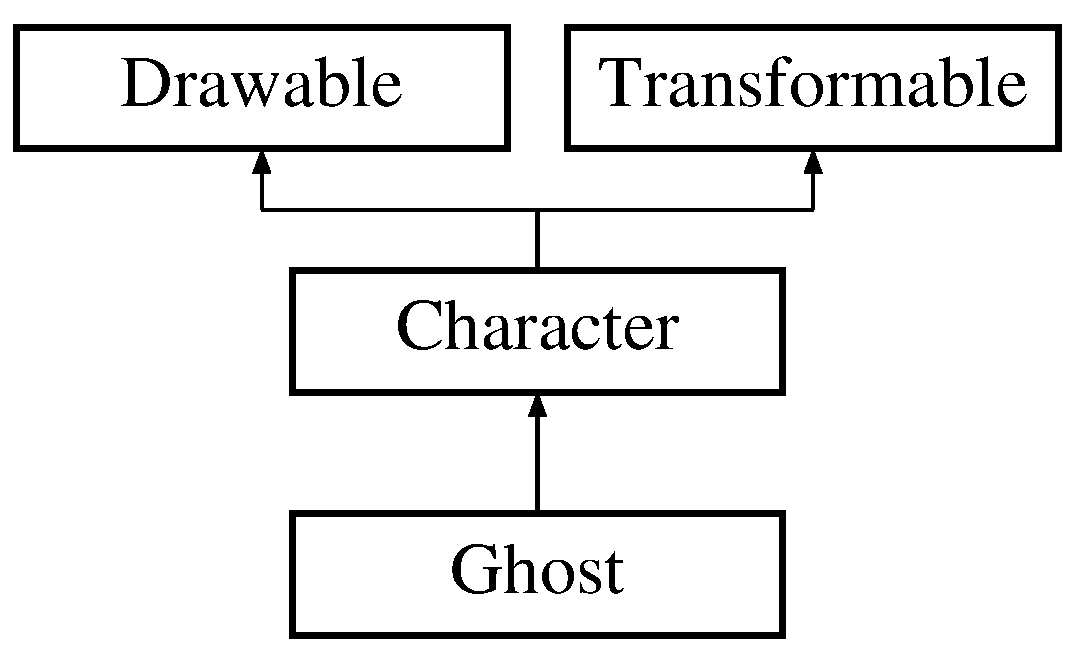
\includegraphics[height=3.000000cm]{class_ghost}
\end{center}
\end{figure}
\subsection*{Public Types}
\begin{DoxyCompactItemize}
\item 
enum \hyperlink{class_ghost_af712fc09f900832a0225928c4556234d}{State} \{ \hyperlink{class_ghost_af712fc09f900832a0225928c4556234dacfaab1cebc10dc849b5e740dad4eb7f0}{Strong}, 
\hyperlink{class_ghost_af712fc09f900832a0225928c4556234da2728b733f9f5d557a05e6fa1aaaf174a}{Weak}
 \}
\end{DoxyCompactItemize}
\subsection*{Public Member Functions}
\begin{DoxyCompactItemize}
\item 
\hyperlink{class_ghost_a931627708b35e6f0b6f9d106adbaee1f}{Ghost} (sf\+::\+Texture \&a\+\_\+texture, \hyperlink{class_pacman}{Pacman} $\ast$a\+\_\+pacman)
\item 
void \hyperlink{class_ghost_ad3af3a46b5c130515dffaae54824341a}{set\+Weak} (sf\+::\+Time a\+\_\+duration)
\item 
bool \hyperlink{class_ghost_af0cf8b5a66a4a390746f43238b96fe55}{is\+Weak} () const
\item 
void \hyperlink{class_ghost_a164e0607f7ea0d72d756bdf964e66b90}{update} (sf\+::\+Time a\+\_\+delta)
\end{DoxyCompactItemize}
\subsection*{Protected Member Functions}
\begin{DoxyCompactItemize}
\item 
void \hyperlink{class_ghost_a08831fa01afa61f91365ce82cf33bf1b}{change\+Direction} ()
\end{DoxyCompactItemize}


\subsection{Detailed Description}
\hyperlink{class_ghost}{Ghost} Class This Class Inherits from the \hyperlink{class_character}{Character} Class. It focuses on the two important ghost attributes\+: the Strong and Weak Animation, and the Pathfinding Algorithm \begin{DoxySeeAlso}{See also}
\hyperlink{class_character}{Character} Claas 
\end{DoxySeeAlso}


\subsection{Member Enumeration Documentation}
\mbox{\Hypertarget{class_ghost_af712fc09f900832a0225928c4556234d}\label{class_ghost_af712fc09f900832a0225928c4556234d}} 
\index{Ghost@{Ghost}!State@{State}}
\index{State@{State}!Ghost@{Ghost}}
\subsubsection{\texorpdfstring{State}{State}}
{\footnotesize\ttfamily enum \hyperlink{class_ghost_af712fc09f900832a0225928c4556234d}{Ghost\+::\+State}}

An enum Type Indicates what state the ghost is in \begin{DoxyEnumFields}{Enumerator}
\raisebox{\heightof{T}}[0pt][0pt]{\index{Strong@{Strong}!Ghost@{Ghost}}\index{Ghost@{Ghost}!Strong@{Strong}}}\mbox{\Hypertarget{class_ghost_af712fc09f900832a0225928c4556234dacfaab1cebc10dc849b5e740dad4eb7f0}\label{class_ghost_af712fc09f900832a0225928c4556234dacfaab1cebc10dc849b5e740dad4eb7f0}} 
Strong&Strong State\+: Can Kill Player \\
\hline

\raisebox{\heightof{T}}[0pt][0pt]{\index{Weak@{Weak}!Ghost@{Ghost}}\index{Ghost@{Ghost}!Weak@{Weak}}}\mbox{\Hypertarget{class_ghost_af712fc09f900832a0225928c4556234da2728b733f9f5d557a05e6fa1aaaf174a}\label{class_ghost_af712fc09f900832a0225928c4556234da2728b733f9f5d557a05e6fa1aaaf174a}} 
Weak&Weak\+State\+: Can be killed by Player \\
\hline

\end{DoxyEnumFields}


\subsection{Constructor \& Destructor Documentation}
\mbox{\Hypertarget{class_ghost_a931627708b35e6f0b6f9d106adbaee1f}\label{class_ghost_a931627708b35e6f0b6f9d106adbaee1f}} 
\index{Ghost@{Ghost}!Ghost@{Ghost}}
\index{Ghost@{Ghost}!Ghost@{Ghost}}
\subsubsection{\texorpdfstring{Ghost()}{Ghost()}}
{\footnotesize\ttfamily Ghost\+::\+Ghost (\begin{DoxyParamCaption}\item[{sf\+::\+Texture \&}]{a\+\_\+texture,  }\item[{\hyperlink{class_pacman}{Pacman} $\ast$}]{a\+\_\+pacman }\end{DoxyParamCaption})}

A \hyperlink{class_ghost}{Ghost} Constructor Initiates the following member variables
\begin{DoxyItemize}
\item m\+\_\+visual
\item m\+\_\+is\+Weak
\item m\+\_\+weak\+State\+Timer
\item m\+\_\+pac\+Man Also uploads animation frames data into the animation sprites
\item m\+\_\+strong\+Animator
\item m\+\_\+weak\+Animator 
\end{DoxyItemize}

\subsection{Member Function Documentation}
\mbox{\Hypertarget{class_ghost_a08831fa01afa61f91365ce82cf33bf1b}\label{class_ghost_a08831fa01afa61f91365ce82cf33bf1b}} 
\index{Ghost@{Ghost}!change\+Direction@{change\+Direction}}
\index{change\+Direction@{change\+Direction}!Ghost@{Ghost}}
\subsubsection{\texorpdfstring{change\+Direction()}{changeDirection()}}
{\footnotesize\ttfamily void Ghost\+::change\+Direction (\begin{DoxyParamCaption}{ }\end{DoxyParamCaption})\hspace{0.3cm}{\ttfamily [protected]}, {\ttfamily [virtual]}}

This function holds the path finding AI for the ghosts. It has a static vector that holds 4 directions and stores it in a map container from best to worst. Gets the angle between pacman and ghost and uses that to decide and rank which direction to take from best to worst if it is in the Strong State. During the Weak State it uses the same ranking but reads it backwards(worst to best). 

Reimplemented from \hyperlink{class_character_ab4c0dc6f72c78607b921cf312e10ed35}{Character}.

\mbox{\Hypertarget{class_ghost_af0cf8b5a66a4a390746f43238b96fe55}\label{class_ghost_af0cf8b5a66a4a390746f43238b96fe55}} 
\index{Ghost@{Ghost}!is\+Weak@{is\+Weak}}
\index{is\+Weak@{is\+Weak}!Ghost@{Ghost}}
\subsubsection{\texorpdfstring{is\+Weak()}{isWeak()}}
{\footnotesize\ttfamily bool Ghost\+::is\+Weak (\begin{DoxyParamCaption}{ }\end{DoxyParamCaption}) const}

This is a get function for m\+\_\+is\+Weak

\begin{DoxyReturn}{Returns}
returns true if the ghost is in the weak state 
\end{DoxyReturn}
\mbox{\Hypertarget{class_ghost_ad3af3a46b5c130515dffaae54824341a}\label{class_ghost_ad3af3a46b5c130515dffaae54824341a}} 
\index{Ghost@{Ghost}!set\+Weak@{set\+Weak}}
\index{set\+Weak@{set\+Weak}!Ghost@{Ghost}}
\subsubsection{\texorpdfstring{set\+Weak()}{setWeak()}}
{\footnotesize\ttfamily void Ghost\+::set\+Weak (\begin{DoxyParamCaption}\item[{sf\+::\+Time}]{a\+\_\+duration }\end{DoxyParamCaption})}

This function set the ghost into the weak state for a certain amount of time which makes it vulnerable to Pac-\/\+Man/\+Quack\+Man Collision


\begin{DoxyParams}{Parameters}
{\em a\+\_\+duration} & the length in sf\+::\+Seconds that the ghost is in wthe weak state \\
\hline
\end{DoxyParams}
\mbox{\Hypertarget{class_ghost_a164e0607f7ea0d72d756bdf964e66b90}\label{class_ghost_a164e0607f7ea0d72d756bdf964e66b90}} 
\index{Ghost@{Ghost}!update@{update}}
\index{update@{update}!Ghost@{Ghost}}
\subsubsection{\texorpdfstring{update()}{update()}}
{\footnotesize\ttfamily void Ghost\+::update (\begin{DoxyParamCaption}\item[{sf\+::\+Time}]{a\+\_\+delta }\end{DoxyParamCaption})\hspace{0.3cm}{\ttfamily [virtual]}}

This function checks the \hyperlink{class_ghost}{Ghost}\textquotesingle{}s current status in game (Dead or Alive) and plays the animation according to it\textquotesingle{}s current state


\begin{DoxyParams}{Parameters}
{\em a\+\_\+delta} & the current time \\
\hline
\end{DoxyParams}


Reimplemented from \hyperlink{class_character_a89b72b507971ba8648909980d045ed06}{Character}.



The documentation for this class was generated from the following files\+:\begin{DoxyCompactItemize}
\item 
\hyperlink{ghost_8hpp}{ghost.\+hpp}\item 
\hyperlink{ghost_8cpp}{ghost.\+cpp}\end{DoxyCompactItemize}

\hypertarget{class_lost_state}{}\section{Lost\+State Class Reference}
\label{class_lost_state}\index{Lost\+State@{Lost\+State}}


{\ttfamily \#include $<$game\+State.\+hpp$>$}

Inheritance diagram for Lost\+State\+:\begin{figure}[H]
\begin{center}
\leavevmode
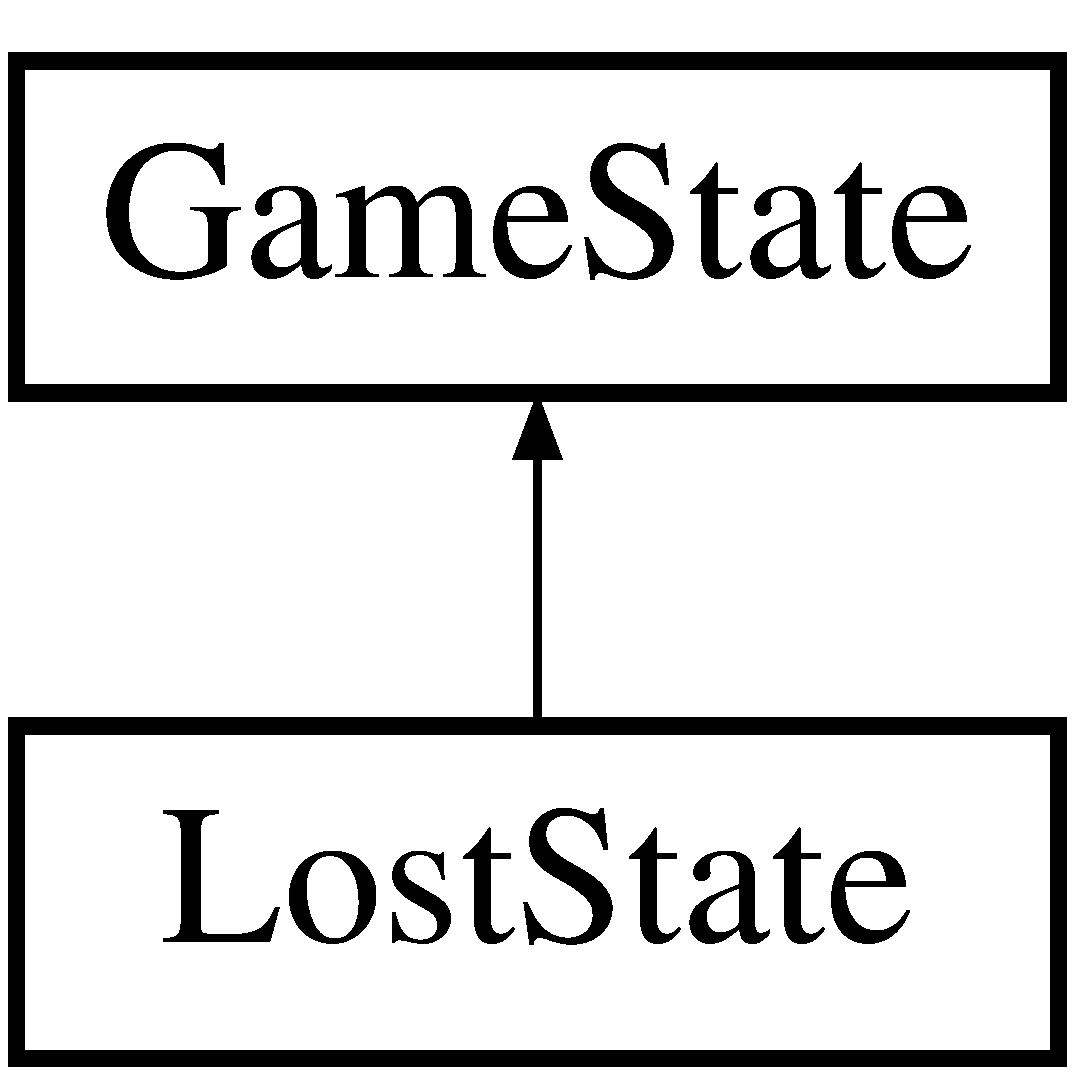
\includegraphics[height=2.000000cm]{class_lost_state}
\end{center}
\end{figure}
\subsection*{Public Member Functions}
\begin{DoxyCompactItemize}
\item 
\hyperlink{class_lost_state_a92bfadd289d793b53b4395510d35f052}{Lost\+State} (\hyperlink{class_game}{Game} $\ast$a\+\_\+game, \hyperlink{class_game_state}{Game\+State} $\ast$a\+\_\+playing\+State)
\item 
void \hyperlink{class_lost_state_aa35179942033d9ab54fbcd7122f40497}{insert\+Coin} ()
\item 
void \hyperlink{class_lost_state_ab0ec749961cfe909dc61289d14444a71}{press\+Button} ()
\item 
void \hyperlink{class_lost_state_abc978a14604451eee5e0373b4ad374c8}{move\+Stick} (sf\+::\+Vector2i a\+\_\+direction)
\item 
void \hyperlink{class_lost_state_a16d5e12284d03f8dd6b25a897b25839b}{update} (sf\+::\+Time a\+\_\+delta)
\item 
void \hyperlink{class_lost_state_acfdefa77d7ed756a1052d39ed2de8786}{draw} (sf\+::\+Render\+Window \&a\+\_\+window)
\end{DoxyCompactItemize}
\subsection*{Additional Inherited Members}


\subsection{Detailed Description}
\hyperlink{class_lost_state}{Lost\+State} Class This Class inherits from the \hyperlink{class_game_state}{Game\+State} Class. This state announces that the player lost the game and is given an option to continue for 10 seconds. If the player chooses to continue, it will give the player another set of lives to play and continue where they left off. If the player chooses to let the timer go down to zero, the game will reset from scratch all the way back to the no coin state. 

Definition at line 448 of file game\+State.\+hpp.



\subsection{Constructor \& Destructor Documentation}
\mbox{\Hypertarget{class_lost_state_a92bfadd289d793b53b4395510d35f052}\label{class_lost_state_a92bfadd289d793b53b4395510d35f052}} 
\index{Lost\+State@{Lost\+State}!Lost\+State@{Lost\+State}}
\index{Lost\+State@{Lost\+State}!Lost\+State@{Lost\+State}}
\subsubsection{\texorpdfstring{Lost\+State()}{LostState()}}
{\footnotesize\ttfamily Lost\+State\+::\+Lost\+State (\begin{DoxyParamCaption}\item[{\hyperlink{class_game}{Game} $\ast$}]{a\+\_\+game,  }\item[{\hyperlink{class_game_state}{Game\+State} $\ast$}]{a\+\_\+playing\+State }\end{DoxyParamCaption})}

A \hyperlink{class_lost_state}{Lost\+State} Constructor Intiates the text to be rendered on the screen and make sures that the score and the maze is kept just incase the player decides to continue 
\begin{DoxyParams}{Parameters}
{\em a\+\_\+game} & the current game instance \\
\hline
{\em a\+\_\+playing\+State} & the current playing\+State entity \\
\hline
\end{DoxyParams}


Definition at line 61 of file game\+State.\+cpp.



\subsection{Member Function Documentation}
\mbox{\Hypertarget{class_lost_state_acfdefa77d7ed756a1052d39ed2de8786}\label{class_lost_state_acfdefa77d7ed756a1052d39ed2de8786}} 
\index{Lost\+State@{Lost\+State}!draw@{draw}}
\index{draw@{draw}!Lost\+State@{Lost\+State}}
\subsubsection{\texorpdfstring{draw()}{draw()}}
{\footnotesize\ttfamily void Lost\+State\+::draw (\begin{DoxyParamCaption}\item[{sf\+::\+Render\+Window \&}]{a\+\_\+window }\end{DoxyParamCaption})\hspace{0.3cm}{\ttfamily [virtual]}}

This function renders the text to the screen


\begin{DoxyParams}{Parameters}
{\em a\+\_\+window} & the window where the game is rendered \\
\hline
\end{DoxyParams}


Implements \hyperlink{class_game_state_a5ffd5ce9acb7499ddef613e8836d1ef8}{Game\+State}.



Definition at line 239 of file game\+State.\+cpp.

\mbox{\Hypertarget{class_lost_state_aa35179942033d9ab54fbcd7122f40497}\label{class_lost_state_aa35179942033d9ab54fbcd7122f40497}} 
\index{Lost\+State@{Lost\+State}!insert\+Coin@{insert\+Coin}}
\index{insert\+Coin@{insert\+Coin}!Lost\+State@{Lost\+State}}
\subsubsection{\texorpdfstring{insert\+Coin()}{insertCoin()}}
{\footnotesize\ttfamily void Lost\+State\+::insert\+Coin (\begin{DoxyParamCaption}{ }\end{DoxyParamCaption})\hspace{0.3cm}{\ttfamily [virtual]}}

This function waits for the player to \char`\"{}insert a coin\char`\"{} and reset the number of lives and resume the current game being played 

Implements \hyperlink{class_game_state_a4cd6f5b4ad23fc08dca287df26d94b94}{Game\+State}.



Definition at line 217 of file game\+State.\+cpp.

\mbox{\Hypertarget{class_lost_state_abc978a14604451eee5e0373b4ad374c8}\label{class_lost_state_abc978a14604451eee5e0373b4ad374c8}} 
\index{Lost\+State@{Lost\+State}!move\+Stick@{move\+Stick}}
\index{move\+Stick@{move\+Stick}!Lost\+State@{Lost\+State}}
\subsubsection{\texorpdfstring{move\+Stick()}{moveStick()}}
{\footnotesize\ttfamily void Lost\+State\+::move\+Stick (\begin{DoxyParamCaption}\item[{sf\+::\+Vector2i}]{a\+\_\+direction }\end{DoxyParamCaption})\hspace{0.3cm}{\ttfamily [virtual]}}

This function sets the direction where Pac-\/\+Man/\+Quack\+Man is going


\begin{DoxyParams}{Parameters}
{\em a\+\_\+direction} & the desired direction \\
\hline
\end{DoxyParams}


Implements \hyperlink{class_game_state_aaae8c1b3ae6969eb2dd81bfc12fbf43f}{Game\+State}.



Definition at line 225 of file game\+State.\+cpp.

\mbox{\Hypertarget{class_lost_state_ab0ec749961cfe909dc61289d14444a71}\label{class_lost_state_ab0ec749961cfe909dc61289d14444a71}} 
\index{Lost\+State@{Lost\+State}!press\+Button@{press\+Button}}
\index{press\+Button@{press\+Button}!Lost\+State@{Lost\+State}}
\subsubsection{\texorpdfstring{press\+Button()}{pressButton()}}
{\footnotesize\ttfamily void Lost\+State\+::press\+Button (\begin{DoxyParamCaption}{ }\end{DoxyParamCaption})\hspace{0.3cm}{\ttfamily [virtual]}}

This is an empty function to override it\textquotesingle{}s virtual counter part \begin{DoxySeeAlso}{See also}
\hyperlink{class_game_state}{Game\+State} Class 
\end{DoxySeeAlso}


Implements \hyperlink{class_game_state_aa14eeaf244bcf19b7013af75cb722dde}{Game\+State}.



Definition at line 222 of file game\+State.\+cpp.

\mbox{\Hypertarget{class_lost_state_a16d5e12284d03f8dd6b25a897b25839b}\label{class_lost_state_a16d5e12284d03f8dd6b25a897b25839b}} 
\index{Lost\+State@{Lost\+State}!update@{update}}
\index{update@{update}!Lost\+State@{Lost\+State}}
\subsubsection{\texorpdfstring{update()}{update()}}
{\footnotesize\ttfamily void Lost\+State\+::update (\begin{DoxyParamCaption}\item[{sf\+::\+Time}]{a\+\_\+delta }\end{DoxyParamCaption})\hspace{0.3cm}{\ttfamily [virtual]}}

This funciton sets a countdown of 10 seconds the shows it to the screen and if the player does not insert a coin within the countdown then it declares \hyperlink{class_game}{Game} Over and the game will reset from scratch and go back to the No Coin State


\begin{DoxyParams}{Parameters}
{\em a\+\_\+delta} & the current time \\
\hline
\end{DoxyParams}


Implements \hyperlink{class_game_state_ab1fe4312f7ce88e7dc11f9935dee67d1}{Game\+State}.



Definition at line 228 of file game\+State.\+cpp.



The documentation for this class was generated from the following files\+:\begin{DoxyCompactItemize}
\item 
smfl\+Test/\hyperlink{game_state_8hpp}{game\+State.\+hpp}\item 
smfl\+Test/\hyperlink{game_state_8cpp}{game\+State.\+cpp}\end{DoxyCompactItemize}

\hypertarget{class_maze}{}\section{Maze Class Reference}
\label{class_maze}\index{Maze@{Maze}}


{\ttfamily \#include $<$maze.\+hpp$>$}

Inheritance diagram for Maze\+:\begin{figure}[H]
\begin{center}
\leavevmode
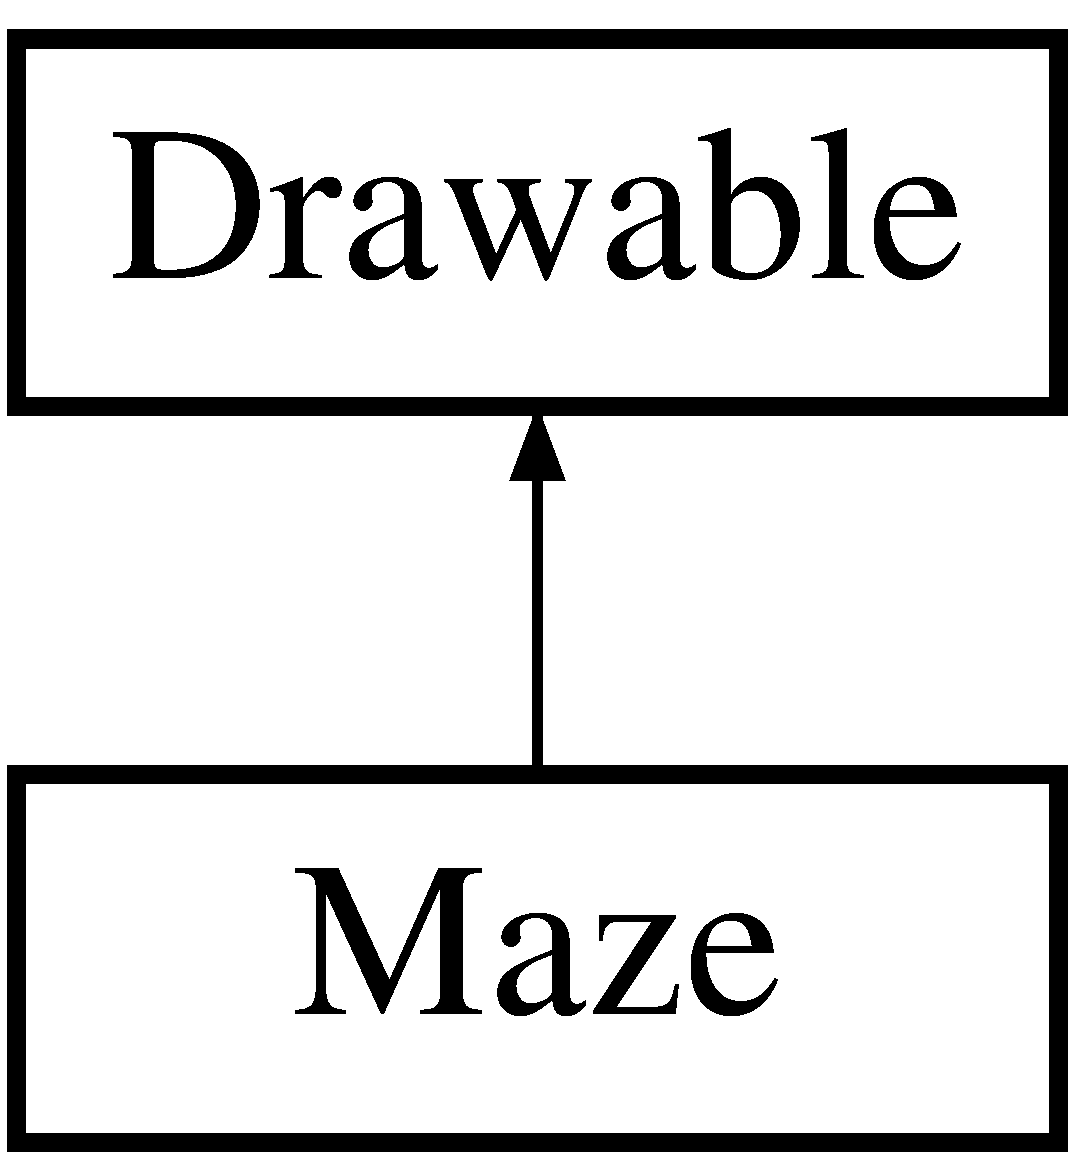
\includegraphics[height=2.000000cm]{class_maze}
\end{center}
\end{figure}
\subsection*{Public Member Functions}
\begin{DoxyCompactItemize}
\item 
\hyperlink{class_maze_a7d8ebd5ec031891fcb2d76d5b8502e44}{Maze} (sf\+::\+Texture \&a\+\_\+texture)
\item 
void \hyperlink{class_maze_a130c9d8858022b05b083a3f0c630fbaf}{load\+Level} (string a\+\_\+file\+Name)
\item 
sf\+::\+Vector2i \hyperlink{class_maze_a664b89e39391a1551babb93556cb36f8}{get\+Size} () const
\item 
sf\+::\+Vector2i \hyperlink{class_maze_a663cb5481d68d68b8d0483d949a125d8}{get\+Pac\+Man\+Position} () const
\item 
vector$<$ sf\+::\+Vector2i $>$ \hyperlink{class_maze_aaf1dc338270b2674df3f5477a512b0a3}{get\+Ghost\+Positions} () const
\item 
sf\+::\+Vector2i \hyperlink{class_maze_a245890f620b8d7ac3445fd4ca0d090e1}{get\+Respawn\+Position} () const
\item 
size\+\_\+t \hyperlink{class_maze_abae2881894d0dcc53d179f74cc7aa3bd}{position\+To\+Index} (sf\+::\+Vector2i a\+\_\+position) const
\item 
sf\+::\+Vector2i \hyperlink{class_maze_ac256166dfc46cc089de0c998295dbc66}{index\+To\+Position} (size\+\_\+t a\+\_\+index) const
\item 
sf\+::\+Vector2i \hyperlink{class_maze_a6e9ed602dba392b5aaf8b694f5aa6197}{map\+Pixel\+To\+Cell} (sf\+::\+Vector2f a\+\_\+pixel) const
\item 
sf\+::\+Vector2f \hyperlink{class_maze_ad1ed938797ff928c0b90cf176d298429}{map\+Cell\+To\+Pixel} (sf\+::\+Vector2i a\+\_\+cell) const
\item 
bool \hyperlink{class_maze_a51a92b406d8376082d6c4f8c67b1490b}{is\+Wall} (sf\+::\+Vector2i a\+\_\+position) const
\item 
bool \hyperlink{class_maze_a26a1d805927e965b54ffa261a87600b9}{is\+Dot} (sf\+::\+Vector2i a\+\_\+position) const
\item 
bool \hyperlink{class_maze_a52450a5ef93f1d11802969587b5ee00d}{is\+Super\+Dot} (sf\+::\+Vector2i a\+\_\+position) const
\item 
bool \hyperlink{class_maze_a63fd7d817f664bb7b157db12479d89be}{is\+Bonus} (sf\+::\+Vector2i a\+\_\+position) const
\item 
void \hyperlink{class_maze_aff24b90af3ab6bd16c94b6831052d3db}{pick\+Object} (sf\+::\+Vector2i a\+\_\+position)
\item 
int \hyperlink{class_maze_afe0905b13aaefd6135346b3cda931556}{get\+Remaining\+Dots} () const
\end{DoxyCompactItemize}


\subsection{Detailed Description}
\hyperlink{class_maze}{Maze} Class This Inherits from sf\+::\+Drawable. It has all the maze methods are handled in this class. The way that the map data are uploaded and stored can be seen here. 

\subsection{Constructor \& Destructor Documentation}
\mbox{\Hypertarget{class_maze_a7d8ebd5ec031891fcb2d76d5b8502e44}\label{class_maze_a7d8ebd5ec031891fcb2d76d5b8502e44}} 
\index{Maze@{Maze}!Maze@{Maze}}
\index{Maze@{Maze}!Maze@{Maze}}
\subsubsection{\texorpdfstring{Maze()}{Maze()}}
{\footnotesize\ttfamily Maze\+::\+Maze (\begin{DoxyParamCaption}\item[{sf\+::\+Texture \&}]{a\+\_\+texture }\end{DoxyParamCaption})}

A \hyperlink{class_maze}{Maze} Consturctor Initiates the following member variables -\/m\+\_\+maze\+Size -\/m\+\_\+texture 

\subsection{Member Function Documentation}
\mbox{\Hypertarget{class_maze_aaf1dc338270b2674df3f5477a512b0a3}\label{class_maze_aaf1dc338270b2674df3f5477a512b0a3}} 
\index{Maze@{Maze}!get\+Ghost\+Positions@{get\+Ghost\+Positions}}
\index{get\+Ghost\+Positions@{get\+Ghost\+Positions}!Maze@{Maze}}
\subsubsection{\texorpdfstring{get\+Ghost\+Positions()}{getGhostPositions()}}
{\footnotesize\ttfamily vector$<$ sf\+::\+Vector2i $>$ Maze\+::get\+Ghost\+Positions (\begin{DoxyParamCaption}{ }\end{DoxyParamCaption}) const}

This funciton is a get function for m\+\_\+ghost\+Positions

\begin{DoxyReturn}{Returns}
returns the vector of the positions of ghost in the maze 
\end{DoxyReturn}
\mbox{\Hypertarget{class_maze_a663cb5481d68d68b8d0483d949a125d8}\label{class_maze_a663cb5481d68d68b8d0483d949a125d8}} 
\index{Maze@{Maze}!get\+Pac\+Man\+Position@{get\+Pac\+Man\+Position}}
\index{get\+Pac\+Man\+Position@{get\+Pac\+Man\+Position}!Maze@{Maze}}
\subsubsection{\texorpdfstring{get\+Pac\+Man\+Position()}{getPacManPosition()}}
{\footnotesize\ttfamily sf\+::\+Vector2i Maze\+::get\+Pac\+Man\+Position (\begin{DoxyParamCaption}{ }\end{DoxyParamCaption}) const}

This function is a get funciton for m\+\_\+pacman\+Position

\begin{DoxyReturn}{Returns}
returns the position of Pac-\/\+Man/\+Quack\+Man in the maze 
\end{DoxyReturn}
\mbox{\Hypertarget{class_maze_afe0905b13aaefd6135346b3cda931556}\label{class_maze_afe0905b13aaefd6135346b3cda931556}} 
\index{Maze@{Maze}!get\+Remaining\+Dots@{get\+Remaining\+Dots}}
\index{get\+Remaining\+Dots@{get\+Remaining\+Dots}!Maze@{Maze}}
\subsubsection{\texorpdfstring{get\+Remaining\+Dots()}{getRemainingDots()}}
{\footnotesize\ttfamily int Maze\+::get\+Remaining\+Dots (\begin{DoxyParamCaption}{ }\end{DoxyParamCaption}) const}

This function is a checks how many dots are left inside the maze

\begin{DoxyReturn}{Returns}
returns the number of dots left in the maze 
\end{DoxyReturn}
\mbox{\Hypertarget{class_maze_a245890f620b8d7ac3445fd4ca0d090e1}\label{class_maze_a245890f620b8d7ac3445fd4ca0d090e1}} 
\index{Maze@{Maze}!get\+Respawn\+Position@{get\+Respawn\+Position}}
\index{get\+Respawn\+Position@{get\+Respawn\+Position}!Maze@{Maze}}
\subsubsection{\texorpdfstring{get\+Respawn\+Position()}{getRespawnPosition()}}
{\footnotesize\ttfamily sf\+::\+Vector2i Maze\+::get\+Respawn\+Position (\begin{DoxyParamCaption}{ }\end{DoxyParamCaption}) const}

This function is a get function for m\+\_\+respawn\+Position

\begin{DoxyReturn}{Returns}
returns the respawn position 
\end{DoxyReturn}
\mbox{\Hypertarget{class_maze_a664b89e39391a1551babb93556cb36f8}\label{class_maze_a664b89e39391a1551babb93556cb36f8}} 
\index{Maze@{Maze}!get\+Size@{get\+Size}}
\index{get\+Size@{get\+Size}!Maze@{Maze}}
\subsubsection{\texorpdfstring{get\+Size()}{getSize()}}
{\footnotesize\ttfamily sf\+::\+Vector2i Maze\+::get\+Size (\begin{DoxyParamCaption}{ }\end{DoxyParamCaption}) const}

This function is a get function for m\+\_\+maze\+Size

\begin{DoxyReturn}{Returns}
returns the size of the map 
\end{DoxyReturn}
\mbox{\Hypertarget{class_maze_ac256166dfc46cc089de0c998295dbc66}\label{class_maze_ac256166dfc46cc089de0c998295dbc66}} 
\index{Maze@{Maze}!index\+To\+Position@{index\+To\+Position}}
\index{index\+To\+Position@{index\+To\+Position}!Maze@{Maze}}
\subsubsection{\texorpdfstring{index\+To\+Position()}{indexToPosition()}}
{\footnotesize\ttfamily sf\+::\+Vector2i Maze\+::index\+To\+Position (\begin{DoxyParamCaption}\item[{size\+\_\+t}]{a\+\_\+index }\end{DoxyParamCaption}) const\hspace{0.3cm}{\ttfamily [inline]}}

This function converts the maze data into the corresponding pixel position in the map


\begin{DoxyParams}{Parameters}
{\em a\+\_\+index} & The maze data \\
\hline
\end{DoxyParams}
\begin{DoxyReturn}{Returns}
returns the pixel position where the maze data is 
\end{DoxyReturn}
\mbox{\Hypertarget{class_maze_a63fd7d817f664bb7b157db12479d89be}\label{class_maze_a63fd7d817f664bb7b157db12479d89be}} 
\index{Maze@{Maze}!is\+Bonus@{is\+Bonus}}
\index{is\+Bonus@{is\+Bonus}!Maze@{Maze}}
\subsubsection{\texorpdfstring{is\+Bonus()}{isBonus()}}
{\footnotesize\ttfamily bool Maze\+::is\+Bonus (\begin{DoxyParamCaption}\item[{sf\+::\+Vector2i}]{a\+\_\+position }\end{DoxyParamCaption}) const}

This function checks if a bonus is on the certain position


\begin{DoxyParams}{Parameters}
{\em a\+\_\+position} & the position to be checked \\
\hline
\end{DoxyParams}
\begin{DoxyReturn}{Returns}
returns true if a bonus is on that position 
\end{DoxyReturn}
\mbox{\Hypertarget{class_maze_a26a1d805927e965b54ffa261a87600b9}\label{class_maze_a26a1d805927e965b54ffa261a87600b9}} 
\index{Maze@{Maze}!is\+Dot@{is\+Dot}}
\index{is\+Dot@{is\+Dot}!Maze@{Maze}}
\subsubsection{\texorpdfstring{is\+Dot()}{isDot()}}
{\footnotesize\ttfamily bool Maze\+::is\+Dot (\begin{DoxyParamCaption}\item[{sf\+::\+Vector2i}]{a\+\_\+position }\end{DoxyParamCaption}) const}

This function checks if a dot/pellet is on the certain position


\begin{DoxyParams}{Parameters}
{\em a\+\_\+position} & the position to be checked \\
\hline
\end{DoxyParams}
\begin{DoxyReturn}{Returns}
returns true if a dot/pellet is on that position 
\end{DoxyReturn}
\mbox{\Hypertarget{class_maze_a52450a5ef93f1d11802969587b5ee00d}\label{class_maze_a52450a5ef93f1d11802969587b5ee00d}} 
\index{Maze@{Maze}!is\+Super\+Dot@{is\+Super\+Dot}}
\index{is\+Super\+Dot@{is\+Super\+Dot}!Maze@{Maze}}
\subsubsection{\texorpdfstring{is\+Super\+Dot()}{isSuperDot()}}
{\footnotesize\ttfamily bool Maze\+::is\+Super\+Dot (\begin{DoxyParamCaption}\item[{sf\+::\+Vector2i}]{a\+\_\+position }\end{DoxyParamCaption}) const}

This function checks if a super dot/pellet is on the certain position


\begin{DoxyParams}{Parameters}
{\em a\+\_\+position} & the position to be checked \\
\hline
\end{DoxyParams}
\begin{DoxyReturn}{Returns}
returns true if a super dot/pellet is on that position 
\end{DoxyReturn}
\mbox{\Hypertarget{class_maze_a51a92b406d8376082d6c4f8c67b1490b}\label{class_maze_a51a92b406d8376082d6c4f8c67b1490b}} 
\index{Maze@{Maze}!is\+Wall@{is\+Wall}}
\index{is\+Wall@{is\+Wall}!Maze@{Maze}}
\subsubsection{\texorpdfstring{is\+Wall()}{isWall()}}
{\footnotesize\ttfamily bool Maze\+::is\+Wall (\begin{DoxyParamCaption}\item[{sf\+::\+Vector2i}]{a\+\_\+position }\end{DoxyParamCaption}) const}

This function checks if a wall is on the certain position


\begin{DoxyParams}{Parameters}
{\em a\+\_\+position} & the position to be checked \\
\hline
\end{DoxyParams}
\begin{DoxyReturn}{Returns}
returns true if a wall is on that position 
\end{DoxyReturn}
\mbox{\Hypertarget{class_maze_a130c9d8858022b05b083a3f0c630fbaf}\label{class_maze_a130c9d8858022b05b083a3f0c630fbaf}} 
\index{Maze@{Maze}!load\+Level@{load\+Level}}
\index{load\+Level@{load\+Level}!Maze@{Maze}}
\subsubsection{\texorpdfstring{load\+Level()}{loadLevel()}}
{\footnotesize\ttfamily void Maze\+::load\+Level (\begin{DoxyParamCaption}\item[{string}]{a\+\_\+file\+Name }\end{DoxyParamCaption})}

This function reads a 28 x 31 image(\+P\+N\+G) which represent the map, then read the pixel data and translate into a vector of sf\+::\+Vector2i. Each color in the image represent certain maze entity. Black are Walls, White are the pellets, Green are the super pellets, Red are the ghost spawn point, Blue is Pac-\/\+Man/\+Quack\+Man\textquotesingle{}s spawn point, and Magenta is the ghost respawn point. This function also takes the maze data and renders wall sprites according to its position (Outer Corner, Inner Corner, Border). 
\begin{DoxyParams}{Parameters}
{\em a\+\_\+file\+Name} & the map image file name \\
\hline
\end{DoxyParams}
\mbox{\Hypertarget{class_maze_ad1ed938797ff928c0b90cf176d298429}\label{class_maze_ad1ed938797ff928c0b90cf176d298429}} 
\index{Maze@{Maze}!map\+Cell\+To\+Pixel@{map\+Cell\+To\+Pixel}}
\index{map\+Cell\+To\+Pixel@{map\+Cell\+To\+Pixel}!Maze@{Maze}}
\subsubsection{\texorpdfstring{map\+Cell\+To\+Pixel()}{mapCellToPixel()}}
{\footnotesize\ttfamily sf\+::\+Vector2f Maze\+::map\+Cell\+To\+Pixel (\begin{DoxyParamCaption}\item[{sf\+::\+Vector2i}]{a\+\_\+cell }\end{DoxyParamCaption}) const}

This function converts a cell value into a pixel value


\begin{DoxyParams}{Parameters}
{\em a\+\_\+cell} & the cell value \\
\hline
\end{DoxyParams}
\begin{DoxyReturn}{Returns}
returns the pixel value that equates to the cell value 
\end{DoxyReturn}
\mbox{\Hypertarget{class_maze_a6e9ed602dba392b5aaf8b694f5aa6197}\label{class_maze_a6e9ed602dba392b5aaf8b694f5aa6197}} 
\index{Maze@{Maze}!map\+Pixel\+To\+Cell@{map\+Pixel\+To\+Cell}}
\index{map\+Pixel\+To\+Cell@{map\+Pixel\+To\+Cell}!Maze@{Maze}}
\subsubsection{\texorpdfstring{map\+Pixel\+To\+Cell()}{mapPixelToCell()}}
{\footnotesize\ttfamily sf\+::\+Vector2i Maze\+::map\+Pixel\+To\+Cell (\begin{DoxyParamCaption}\item[{sf\+::\+Vector2f}]{a\+\_\+pixel }\end{DoxyParamCaption}) const}

This function converts a pixel value into a cell value


\begin{DoxyParams}{Parameters}
{\em a\+\_\+pixel} & the pixel value \\
\hline
\end{DoxyParams}
\begin{DoxyReturn}{Returns}
returns the cell value that equates to the pixel value 
\end{DoxyReturn}
\mbox{\Hypertarget{class_maze_aff24b90af3ab6bd16c94b6831052d3db}\label{class_maze_aff24b90af3ab6bd16c94b6831052d3db}} 
\index{Maze@{Maze}!pick\+Object@{pick\+Object}}
\index{pick\+Object@{pick\+Object}!Maze@{Maze}}
\subsubsection{\texorpdfstring{pick\+Object()}{pickObject()}}
{\footnotesize\ttfamily void Maze\+::pick\+Object (\begin{DoxyParamCaption}\item[{sf\+::\+Vector2i}]{a\+\_\+position }\end{DoxyParamCaption})}

This function sets the dot, super dot, and bonus as Empty in the maze data after collision, and also make sures that it does not set the walls to empty after collition


\begin{DoxyParams}{Parameters}
{\em a\+\_\+position} & the position where the player is \\
\hline
\end{DoxyParams}
\mbox{\Hypertarget{class_maze_abae2881894d0dcc53d179f74cc7aa3bd}\label{class_maze_abae2881894d0dcc53d179f74cc7aa3bd}} 
\index{Maze@{Maze}!position\+To\+Index@{position\+To\+Index}}
\index{position\+To\+Index@{position\+To\+Index}!Maze@{Maze}}
\subsubsection{\texorpdfstring{position\+To\+Index()}{positionToIndex()}}
{\footnotesize\ttfamily size\+\_\+t Maze\+::position\+To\+Index (\begin{DoxyParamCaption}\item[{sf\+::\+Vector2i}]{a\+\_\+position }\end{DoxyParamCaption}) const\hspace{0.3cm}{\ttfamily [inline]}}

This function converts the pixel position into the corresponding maze data


\begin{DoxyParams}{Parameters}
{\em a\+\_\+position} & The pixel position \\
\hline
\end{DoxyParams}
\begin{DoxyReturn}{Returns}
returns the maze data that matches the position 
\end{DoxyReturn}


The documentation for this class was generated from the following files\+:\begin{DoxyCompactItemize}
\item 
\hyperlink{maze_8hpp}{maze.\+hpp}\item 
\hyperlink{maze_8cpp}{maze.\+cpp}\end{DoxyCompactItemize}

\hypertarget{class_no_coin_state}{}\section{No\+Coin\+State Class Reference}
\label{class_no_coin_state}\index{No\+Coin\+State@{No\+Coin\+State}}


{\ttfamily \#include $<$game\+State.\+hpp$>$}

Inheritance diagram for No\+Coin\+State\+:\begin{figure}[H]
\begin{center}
\leavevmode
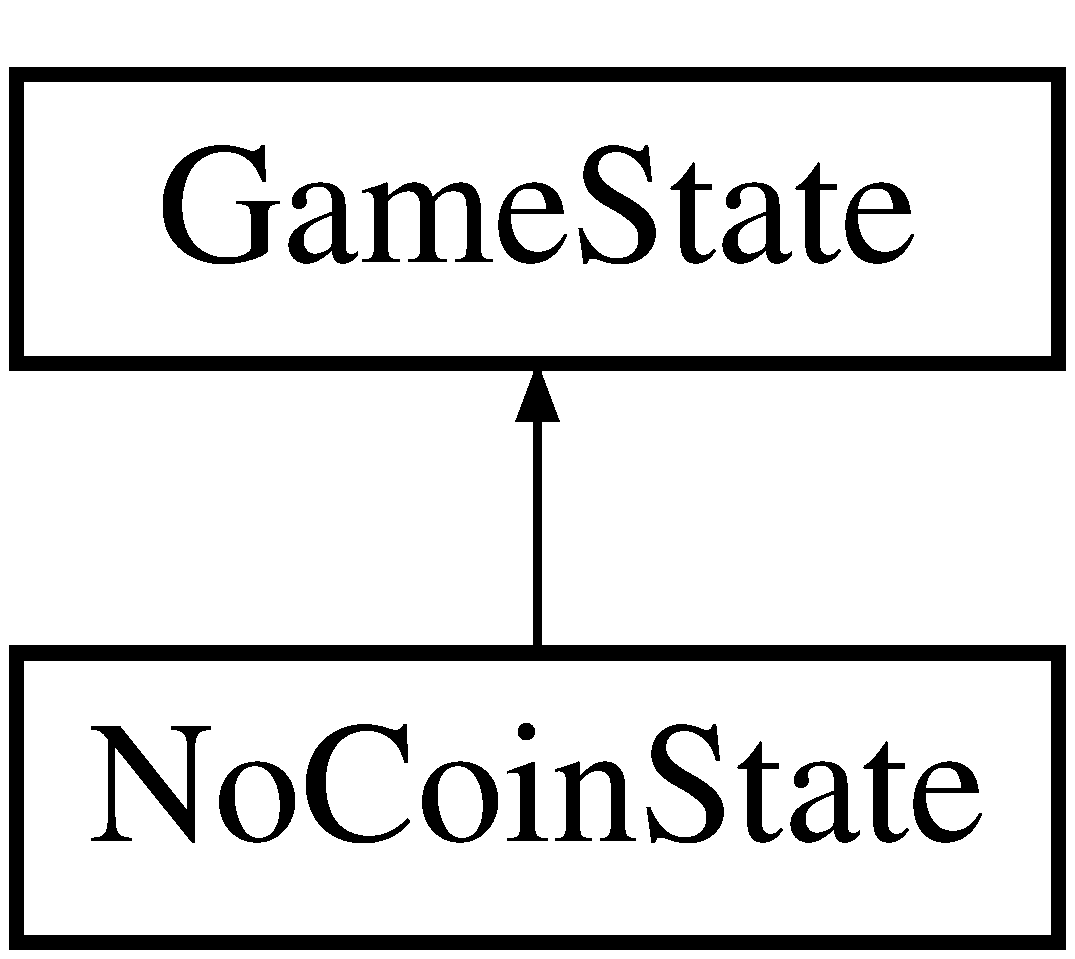
\includegraphics[height=2.000000cm]{class_no_coin_state}
\end{center}
\end{figure}
\subsection*{Public Member Functions}
\begin{DoxyCompactItemize}
\item 
\hyperlink{class_no_coin_state_a3c0129051f00eb142a2055e181264549}{No\+Coin\+State} (\hyperlink{class_game}{Game} $\ast$a\+\_\+game)
\item 
void \hyperlink{class_no_coin_state_a417209eadad2f71284cf09d369bc389e}{insert\+Coin} ()
\item 
void \hyperlink{class_no_coin_state_a47dd2924ce9601b45ee11e0d9b8452f7}{press\+Button} ()
\item 
void \hyperlink{class_no_coin_state_a9fe8f36082705e6f5833244890093adc}{move\+Stick} (sf\+::\+Vector2i a\+\_\+direction)
\item 
void \hyperlink{class_no_coin_state_af0194851310c6df176770713341a8b80}{update} (sf\+::\+Time a\+\_\+delta)
\item 
void \hyperlink{class_no_coin_state_ab1e920e22b90f9d36954e75ea49c3f9b}{draw} (sf\+::\+Render\+Window \&a\+\_\+window)
\end{DoxyCompactItemize}
\subsection*{Additional Inherited Members}


\subsection{Detailed Description}
\hyperlink{class_no_coin_state}{No\+Coin\+State} Class This class inherits from the \hyperlink{class_game_state}{Game\+State} Class. This game state activates when the game is first launches and also when the player chooses not to continue. 

\subsection{Constructor \& Destructor Documentation}
\mbox{\Hypertarget{class_no_coin_state_a3c0129051f00eb142a2055e181264549}\label{class_no_coin_state_a3c0129051f00eb142a2055e181264549}} 
\index{No\+Coin\+State@{No\+Coin\+State}!No\+Coin\+State@{No\+Coin\+State}}
\index{No\+Coin\+State@{No\+Coin\+State}!No\+Coin\+State@{No\+Coin\+State}}
\subsubsection{\texorpdfstring{No\+Coin\+State()}{NoCoinState()}}
{\footnotesize\ttfamily No\+Coin\+State\+::\+No\+Coin\+State (\begin{DoxyParamCaption}\item[{\hyperlink{class_game}{Game} $\ast$}]{a\+\_\+game }\end{DoxyParamCaption})}

A \hyperlink{class_no_coin_state}{No\+Coin\+State} Constructor Intiates the game logo, font, and the texts to be rendered on the screen 
\begin{DoxyParams}{Parameters}
{\em a\+\_\+game} & the current game instance \\
\hline
\end{DoxyParams}


\subsection{Member Function Documentation}
\mbox{\Hypertarget{class_no_coin_state_ab1e920e22b90f9d36954e75ea49c3f9b}\label{class_no_coin_state_ab1e920e22b90f9d36954e75ea49c3f9b}} 
\index{No\+Coin\+State@{No\+Coin\+State}!draw@{draw}}
\index{draw@{draw}!No\+Coin\+State@{No\+Coin\+State}}
\subsubsection{\texorpdfstring{draw()}{draw()}}
{\footnotesize\ttfamily void No\+Coin\+State\+::draw (\begin{DoxyParamCaption}\item[{sf\+::\+Render\+Window \&}]{a\+\_\+window }\end{DoxyParamCaption})\hspace{0.3cm}{\ttfamily [virtual]}}

This function renders game logo and renders the text only if m\+\_\+display\+Text is true which gives the blinking effect


\begin{DoxyParams}{Parameters}
{\em a\+\_\+window} & the window where the game is rendered \\
\hline
\end{DoxyParams}


Implements \hyperlink{class_game_state_a5ffd5ce9acb7499ddef613e8836d1ef8}{Game\+State}.

\mbox{\Hypertarget{class_no_coin_state_a417209eadad2f71284cf09d369bc389e}\label{class_no_coin_state_a417209eadad2f71284cf09d369bc389e}} 
\index{No\+Coin\+State@{No\+Coin\+State}!insert\+Coin@{insert\+Coin}}
\index{insert\+Coin@{insert\+Coin}!No\+Coin\+State@{No\+Coin\+State}}
\subsubsection{\texorpdfstring{insert\+Coin()}{insertCoin()}}
{\footnotesize\ttfamily void No\+Coin\+State\+::insert\+Coin (\begin{DoxyParamCaption}{ }\end{DoxyParamCaption})\hspace{0.3cm}{\ttfamily [virtual]}}

This function changes the current game\textquotesingle{}s state to the get ready state \begin{DoxySeeAlso}{See also}
\hyperlink{class_game_state}{Game\+State} Class 
\end{DoxySeeAlso}


Implements \hyperlink{class_game_state_a4cd6f5b4ad23fc08dca287df26d94b94}{Game\+State}.

\mbox{\Hypertarget{class_no_coin_state_a9fe8f36082705e6f5833244890093adc}\label{class_no_coin_state_a9fe8f36082705e6f5833244890093adc}} 
\index{No\+Coin\+State@{No\+Coin\+State}!move\+Stick@{move\+Stick}}
\index{move\+Stick@{move\+Stick}!No\+Coin\+State@{No\+Coin\+State}}
\subsubsection{\texorpdfstring{move\+Stick()}{moveStick()}}
{\footnotesize\ttfamily void No\+Coin\+State\+::move\+Stick (\begin{DoxyParamCaption}\item[{sf\+::\+Vector2i}]{a\+\_\+direction }\end{DoxyParamCaption})\hspace{0.3cm}{\ttfamily [virtual]}}

This is an empty function to override it\textquotesingle{}s virtual counter part \begin{DoxySeeAlso}{See also}
\hyperlink{class_game_state}{Game\+State} Class 
\end{DoxySeeAlso}

\begin{DoxyParams}{Parameters}
{\em a\+\_\+direction} & the desired direction \\
\hline
\end{DoxyParams}


Implements \hyperlink{class_game_state_aaae8c1b3ae6969eb2dd81bfc12fbf43f}{Game\+State}.

\mbox{\Hypertarget{class_no_coin_state_a47dd2924ce9601b45ee11e0d9b8452f7}\label{class_no_coin_state_a47dd2924ce9601b45ee11e0d9b8452f7}} 
\index{No\+Coin\+State@{No\+Coin\+State}!press\+Button@{press\+Button}}
\index{press\+Button@{press\+Button}!No\+Coin\+State@{No\+Coin\+State}}
\subsubsection{\texorpdfstring{press\+Button()}{pressButton()}}
{\footnotesize\ttfamily void No\+Coin\+State\+::press\+Button (\begin{DoxyParamCaption}{ }\end{DoxyParamCaption})\hspace{0.3cm}{\ttfamily [virtual]}}

This is an empty function to override it\textquotesingle{}s virtual counter part \begin{DoxySeeAlso}{See also}
\hyperlink{class_game_state}{Game\+State} Class 
\end{DoxySeeAlso}


Implements \hyperlink{class_game_state_aa14eeaf244bcf19b7013af75cb722dde}{Game\+State}.

\mbox{\Hypertarget{class_no_coin_state_af0194851310c6df176770713341a8b80}\label{class_no_coin_state_af0194851310c6df176770713341a8b80}} 
\index{No\+Coin\+State@{No\+Coin\+State}!update@{update}}
\index{update@{update}!No\+Coin\+State@{No\+Coin\+State}}
\subsubsection{\texorpdfstring{update()}{update()}}
{\footnotesize\ttfamily void No\+Coin\+State\+::update (\begin{DoxyParamCaption}\item[{sf\+::\+Time}]{a\+\_\+delta }\end{DoxyParamCaption})\hspace{0.3cm}{\ttfamily [virtual]}}

This function updates the window which renders the game logo and the blinking \char`\"{}insert coin\char`\"{} text


\begin{DoxyParams}{Parameters}
{\em a\+\_\+delta} & the current time \\
\hline
\end{DoxyParams}


Implements \hyperlink{class_game_state_ab1fe4312f7ce88e7dc11f9935dee67d1}{Game\+State}.



The documentation for this class was generated from the following files\+:\begin{DoxyCompactItemize}
\item 
\hyperlink{game_state_8hpp}{game\+State.\+hpp}\item 
\hyperlink{game_state_8cpp}{game\+State.\+cpp}\end{DoxyCompactItemize}

\hypertarget{class_pacman}{}\section{Pacman Class Reference}
\label{class_pacman}\index{Pacman@{Pacman}}


{\ttfamily \#include $<$pacman.\+hpp$>$}

Inheritance diagram for Pacman\+:\begin{figure}[H]
\begin{center}
\leavevmode
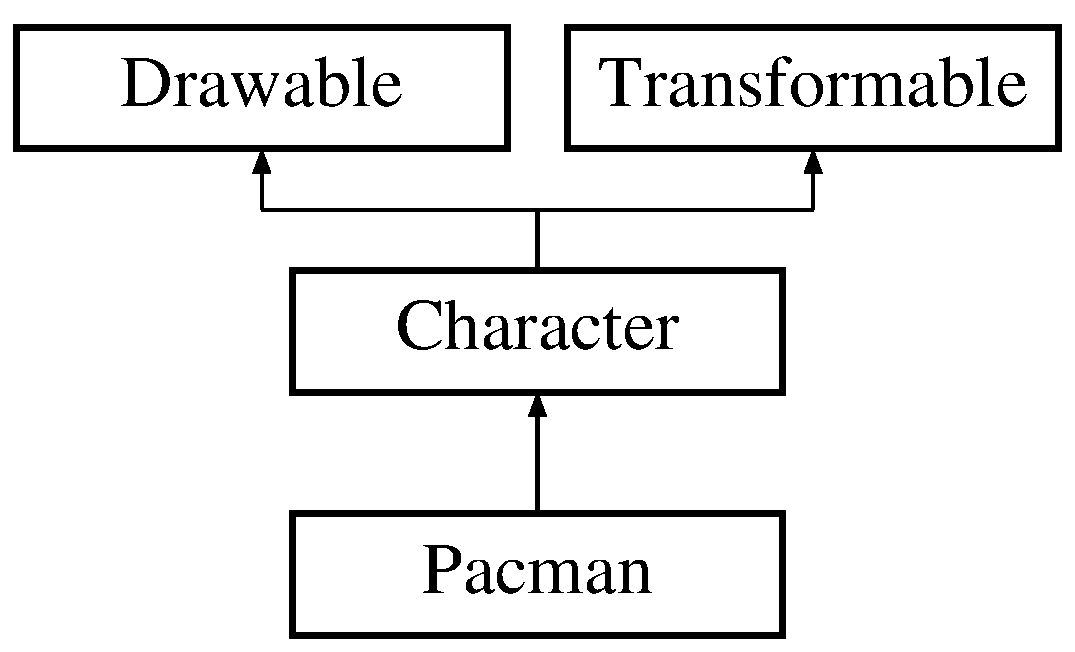
\includegraphics[height=3.000000cm]{class_pacman}
\end{center}
\end{figure}
\subsection*{Public Member Functions}
\begin{DoxyCompactItemize}
\item 
\hyperlink{class_pacman_a7be693fb4bf4dc49ede1f022e79022e0}{Pacman} (sf\+::\+Texture \&a\+\_\+texture)
\item 
void \hyperlink{class_pacman_a880f3f899b2f2d1ee9969fa049f7289d}{die} ()
\item 
bool \hyperlink{class_pacman_afefb1eac50a96a7449ee8e910688614e}{is\+Dying} () const
\item 
bool \hyperlink{class_pacman_a5f0f0398fc20f7c06c5f05a20ad2c1ed}{is\+Dead} () const
\item 
void \hyperlink{class_pacman_a6badb47a28223991a1eb540f9d970e77}{update} (sf\+::\+Time a\+\_\+delta)
\item 
void \hyperlink{class_pacman_a6b190109b2d9400c4eb7c52913ffd0c6}{reset} ()
\end{DoxyCompactItemize}
\subsection*{Additional Inherited Members}


\subsection{Detailed Description}
\hyperlink{class_pacman}{Pacman} Class This Class Inherits from the \hyperlink{class_character}{Character} Class. It focuses on all of Pac-\/\+Man/\+Quack\+Man\textquotesingle{}s attributes and behavior such as, Animation Sprites, Running and Dying Animation, and Death. \begin{DoxySeeAlso}{See also}
\hyperlink{class_character}{Character} Class 
\end{DoxySeeAlso}


Definition at line 22 of file pacman.\+hpp.



\subsection{Constructor \& Destructor Documentation}
\mbox{\Hypertarget{class_pacman_a7be693fb4bf4dc49ede1f022e79022e0}\label{class_pacman_a7be693fb4bf4dc49ede1f022e79022e0}} 
\index{Pacman@{Pacman}!Pacman@{Pacman}}
\index{Pacman@{Pacman}!Pacman@{Pacman}}
\subsubsection{\texorpdfstring{Pacman()}{Pacman()}}
{\footnotesize\ttfamily Pacman\+::\+Pacman (\begin{DoxyParamCaption}\item[{sf\+::\+Texture \&}]{a\+\_\+texture }\end{DoxyParamCaption})}

A \hyperlink{class_pacman}{Pacman} Constructor Initiates the following member variables
\begin{DoxyItemize}
\item m\+\_\+visual
\item m\+\_\+is\+Dead
\item m\+\_\+is\+Dying Also uploads animation frames data into the animation sprites
\item m\+\_\+run\+Animator
\item m\+\_\+die\+Animator
\end{DoxyItemize}


\begin{DoxyParams}{Parameters}
{\em a\+\_\+texture} & the texture sheet \\
\hline
\end{DoxyParams}


Definition at line 11 of file pacman.\+cpp.



\subsection{Member Function Documentation}
\mbox{\Hypertarget{class_pacman_a880f3f899b2f2d1ee9969fa049f7289d}\label{class_pacman_a880f3f899b2f2d1ee9969fa049f7289d}} 
\index{Pacman@{Pacman}!die@{die}}
\index{die@{die}!Pacman@{Pacman}}
\subsubsection{\texorpdfstring{die()}{die()}}
{\footnotesize\ttfamily void Pacman\+::die (\begin{DoxyParamCaption}{ }\end{DoxyParamCaption})}

This function ensure that the Pac-\/\+Man/\+Quack\+Man death animation plays and indicate that Player is dead 

Definition at line 35 of file pacman.\+cpp.

\mbox{\Hypertarget{class_pacman_a5f0f0398fc20f7c06c5f05a20ad2c1ed}\label{class_pacman_a5f0f0398fc20f7c06c5f05a20ad2c1ed}} 
\index{Pacman@{Pacman}!is\+Dead@{is\+Dead}}
\index{is\+Dead@{is\+Dead}!Pacman@{Pacman}}
\subsubsection{\texorpdfstring{is\+Dead()}{isDead()}}
{\footnotesize\ttfamily bool Pacman\+::is\+Dead (\begin{DoxyParamCaption}{ }\end{DoxyParamCaption}) const}

This function is a get function for m\+\_\+is\+Dead

\begin{DoxyReturn}{Returns}
returns whether the player is dead or not 
\end{DoxyReturn}


Definition at line 45 of file pacman.\+cpp.

\mbox{\Hypertarget{class_pacman_afefb1eac50a96a7449ee8e910688614e}\label{class_pacman_afefb1eac50a96a7449ee8e910688614e}} 
\index{Pacman@{Pacman}!is\+Dying@{is\+Dying}}
\index{is\+Dying@{is\+Dying}!Pacman@{Pacman}}
\subsubsection{\texorpdfstring{is\+Dying()}{isDying()}}
{\footnotesize\ttfamily bool Pacman\+::is\+Dying (\begin{DoxyParamCaption}{ }\end{DoxyParamCaption}) const}

This function is a get function for m\+\_\+is\+Dying

\begin{DoxyReturn}{Returns}
returns true dying animation is currently playing 
\end{DoxyReturn}


Definition at line 42 of file pacman.\+cpp.

\mbox{\Hypertarget{class_pacman_a6b190109b2d9400c4eb7c52913ffd0c6}\label{class_pacman_a6b190109b2d9400c4eb7c52913ffd0c6}} 
\index{Pacman@{Pacman}!reset@{reset}}
\index{reset@{reset}!Pacman@{Pacman}}
\subsubsection{\texorpdfstring{reset()}{reset()}}
{\footnotesize\ttfamily void Pacman\+::reset (\begin{DoxyParamCaption}{ }\end{DoxyParamCaption})}

This function restarts Pac-\/\+Man/\+Quack\+Man\textquotesingle{}s Animation back to it\textquotesingle{}s running state 

Definition at line 49 of file pacman.\+cpp.

\mbox{\Hypertarget{class_pacman_a6badb47a28223991a1eb540f9d970e77}\label{class_pacman_a6badb47a28223991a1eb540f9d970e77}} 
\index{Pacman@{Pacman}!update@{update}}
\index{update@{update}!Pacman@{Pacman}}
\subsubsection{\texorpdfstring{update()}{update()}}
{\footnotesize\ttfamily void Pacman\+::update (\begin{DoxyParamCaption}\item[{sf\+::\+Time}]{a\+\_\+delta }\end{DoxyParamCaption})\hspace{0.3cm}{\ttfamily [virtual]}}

This function checks the Player\textquotesingle{}s current status in game (Dead or Alive) and plays the animation according to it\textquotesingle{}s current state


\begin{DoxyParams}{Parameters}
{\em a\+\_\+delta} & the current time \\
\hline
\end{DoxyParams}


Reimplemented from \hyperlink{class_character_a89b72b507971ba8648909980d045ed06}{Character}.



Definition at line 63 of file pacman.\+cpp.



The documentation for this class was generated from the following files\+:\begin{DoxyCompactItemize}
\item 
smfl\+Test/\hyperlink{pacman_8hpp}{pacman.\+hpp}\item 
smfl\+Test/\hyperlink{pacman_8cpp}{pacman.\+cpp}\end{DoxyCompactItemize}

\hypertarget{class_playing_state}{}\section{Playing\+State Class Reference}
\label{class_playing_state}\index{Playing\+State@{Playing\+State}}


{\ttfamily \#include $<$game\+State.\+hpp$>$}

Inheritance diagram for Playing\+State\+:\begin{figure}[H]
\begin{center}
\leavevmode
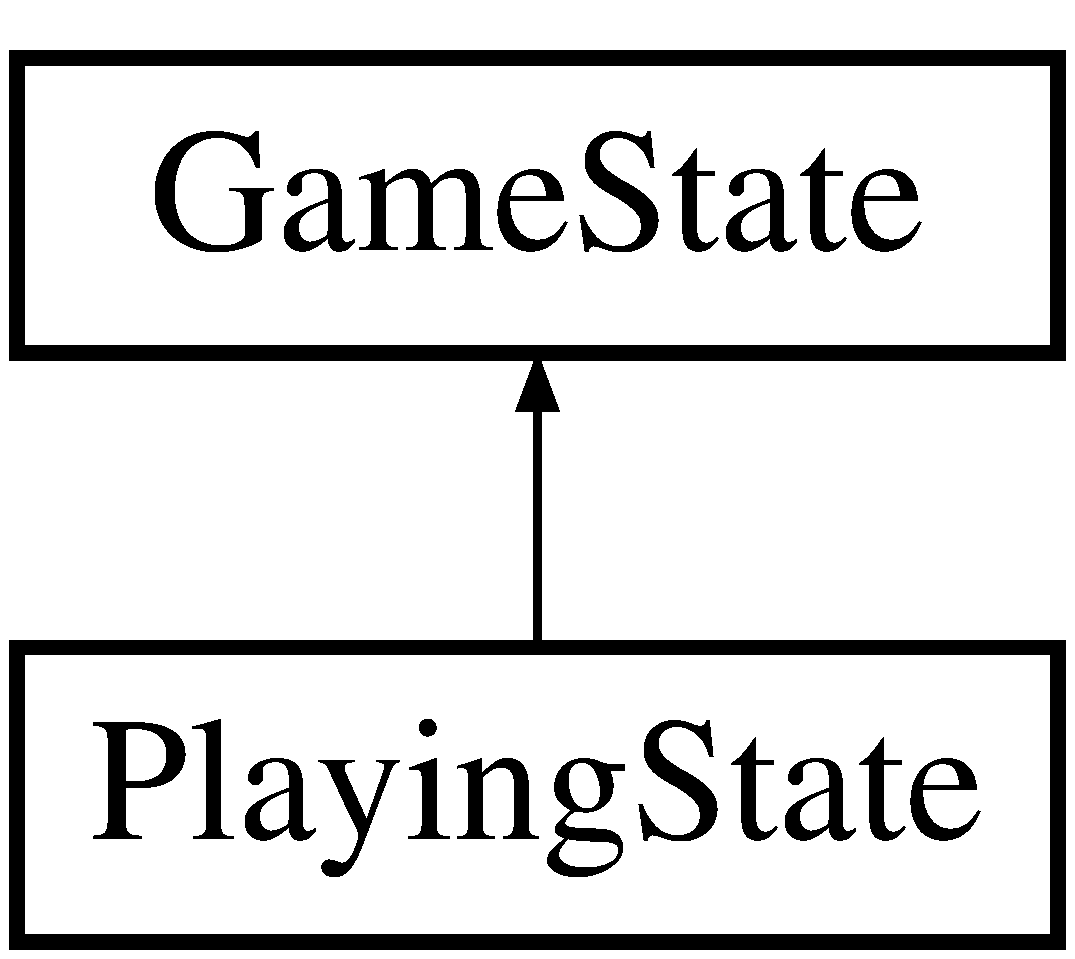
\includegraphics[height=2.000000cm]{class_playing_state}
\end{center}
\end{figure}
\subsection*{Public Member Functions}
\begin{DoxyCompactItemize}
\item 
\hyperlink{class_playing_state_a09c8d3c87687ffa4e5f04c70265d67de}{Playing\+State} (\hyperlink{class_game}{Game} $\ast$a\+\_\+game)
\item 
\hyperlink{class_playing_state_afd96eb2be532e40c9db2f9607e4ea284}{$\sim$\+Playing\+State} ()
\item 
void \hyperlink{class_playing_state_a936d41a2041ace2ccb67a9b779d113a7}{insert\+Coin} ()
\item 
void \hyperlink{class_playing_state_ae59ff244a6cd4a3c6f6fcaef41f4d8c5}{press\+Button} ()
\item 
void \hyperlink{class_playing_state_af205fbb130a2c83b260d80359de914e8}{move\+Stick} (sf\+::\+Vector2i a\+\_\+direction)
\item 
void \hyperlink{class_playing_state_a62b3904b8a971fed2f8fab4eb73bd9e5}{update} (sf\+::\+Time a\+\_\+delta)
\item 
void \hyperlink{class_playing_state_aa6c7033a5c734ba1ae4aae0905554d61}{draw} (sf\+::\+Render\+Window \&a\+\_\+window)
\item 
void \hyperlink{class_playing_state_a18ea22c1b551f6d81d030853f8ce9b73}{load\+Next\+Lvl} ()
\item 
void \hyperlink{class_playing_state_ac2093c243cc85bb767b27797060aab2c}{game\+Over} ()
\item 
void \hyperlink{class_playing_state_a464c879dc893195b041efa58b3b3e73f}{reset\+Lives} ()
\item 
void \hyperlink{class_playing_state_a11a3e0a2d479e659c442deb9c87fdeed}{reset\+Current\+Lvl} ()
\item 
void \hyperlink{class_playing_state_ac1d69f92915e66c4335c6218c0837179}{reset\+Characters} ()
\item 
int \hyperlink{class_playing_state_ab07b1a4993541b38e81f756ac0f4e46b}{get\+Score} ()
\end{DoxyCompactItemize}
\subsection*{Additional Inherited Members}


\subsection{Detailed Description}
Playing State Class This class inherits from the \hyperlink{class_game_state}{Game\+State} Class. This game state is where everything is implemented. The game is played in this state. It takes care of loading the levels, calculating scores, checking for Player VS \hyperlink{class_ghost}{Ghost} Collisions, picking up pellets, and rendering the H\+UD. 

Definition at line 219 of file game\+State.\+hpp.



\subsection{Constructor \& Destructor Documentation}
\mbox{\Hypertarget{class_playing_state_a09c8d3c87687ffa4e5f04c70265d67de}\label{class_playing_state_a09c8d3c87687ffa4e5f04c70265d67de}} 
\index{Playing\+State@{Playing\+State}!Playing\+State@{Playing\+State}}
\index{Playing\+State@{Playing\+State}!Playing\+State@{Playing\+State}}
\subsubsection{\texorpdfstring{Playing\+State()}{PlayingState()}}
{\footnotesize\ttfamily Playing\+State\+::\+Playing\+State (\begin{DoxyParamCaption}\item[{\hyperlink{class_game}{Game} $\ast$}]{a\+\_\+game }\end{DoxyParamCaption})}

A \hyperlink{class_playing_state}{Playing\+State} Constructor Intiates the following member variables
\begin{DoxyItemize}
\item m\+\_\+maze
\item m\+\_\+bonus
\item m\+\_\+pac\+Man
\item m\+\_\+lvl
\item m\+\_\+lives
\item m\+\_\+score Also sets up everything on the maze and prepares all the H\+UD elements to be rendered to the screen 
\begin{DoxyParams}{Parameters}
{\em the} & current game instance \\
\hline
\end{DoxyParams}

\end{DoxyItemize}

Definition at line 84 of file game\+State.\+cpp.

\mbox{\Hypertarget{class_playing_state_afd96eb2be532e40c9db2f9607e4ea284}\label{class_playing_state_afd96eb2be532e40c9db2f9607e4ea284}} 
\index{Playing\+State@{Playing\+State}!````~Playing\+State@{$\sim$\+Playing\+State}}
\index{````~Playing\+State@{$\sim$\+Playing\+State}!Playing\+State@{Playing\+State}}
\subsubsection{\texorpdfstring{$\sim$\+Playing\+State()}{~PlayingState()}}
{\footnotesize\ttfamily Playing\+State\+::$\sim$\+Playing\+State (\begin{DoxyParamCaption}{ }\end{DoxyParamCaption})}

A \hyperlink{class_playing_state}{Playing\+State} Destructor Deletes the current instances of Pac-\/\+Man/\+Quack\+Man and ghosts 

Definition at line 134 of file game\+State.\+cpp.



\subsection{Member Function Documentation}
\mbox{\Hypertarget{class_playing_state_aa6c7033a5c734ba1ae4aae0905554d61}\label{class_playing_state_aa6c7033a5c734ba1ae4aae0905554d61}} 
\index{Playing\+State@{Playing\+State}!draw@{draw}}
\index{draw@{draw}!Playing\+State@{Playing\+State}}
\subsubsection{\texorpdfstring{draw()}{draw()}}
{\footnotesize\ttfamily void Playing\+State\+::draw (\begin{DoxyParamCaption}\item[{sf\+::\+Render\+Window \&}]{a\+\_\+window }\end{DoxyParamCaption})\hspace{0.3cm}{\ttfamily [virtual]}}

This functions draws everything on the screen. The \hyperlink{class_maze}{Maze}, Pac-\/\+Man/\+Quack\+Man, The ghosts, and the H\+UD


\begin{DoxyParams}{Parameters}
{\em a\+\_\+window} & the window where the game is rendered \\
\hline
\end{DoxyParams}


Implements \hyperlink{class_game_state_a5ffd5ce9acb7499ddef613e8836d1ef8}{Game\+State}.



Definition at line 329 of file game\+State.\+cpp.

\mbox{\Hypertarget{class_playing_state_ac2093c243cc85bb767b27797060aab2c}\label{class_playing_state_ac2093c243cc85bb767b27797060aab2c}} 
\index{Playing\+State@{Playing\+State}!game\+Over@{game\+Over}}
\index{game\+Over@{game\+Over}!Playing\+State@{Playing\+State}}
\subsubsection{\texorpdfstring{game\+Over()}{gameOver()}}
{\footnotesize\ttfamily void Playing\+State\+::game\+Over (\begin{DoxyParamCaption}{ }\end{DoxyParamCaption})}

This function resets all the in game variables. Set everything like a new game 

Definition at line 409 of file game\+State.\+cpp.

\mbox{\Hypertarget{class_playing_state_ab07b1a4993541b38e81f756ac0f4e46b}\label{class_playing_state_ab07b1a4993541b38e81f756ac0f4e46b}} 
\index{Playing\+State@{Playing\+State}!get\+Score@{get\+Score}}
\index{get\+Score@{get\+Score}!Playing\+State@{Playing\+State}}
\subsubsection{\texorpdfstring{get\+Score()}{getScore()}}
{\footnotesize\ttfamily int Playing\+State\+::get\+Score (\begin{DoxyParamCaption}{ }\end{DoxyParamCaption})}

This is a get function for m\+\_\+score;

\begin{DoxyReturn}{Returns}
returns the current game score 
\end{DoxyReturn}


Definition at line 427 of file game\+State.\+cpp.

\mbox{\Hypertarget{class_playing_state_a936d41a2041ace2ccb67a9b779d113a7}\label{class_playing_state_a936d41a2041ace2ccb67a9b779d113a7}} 
\index{Playing\+State@{Playing\+State}!insert\+Coin@{insert\+Coin}}
\index{insert\+Coin@{insert\+Coin}!Playing\+State@{Playing\+State}}
\subsubsection{\texorpdfstring{insert\+Coin()}{insertCoin()}}
{\footnotesize\ttfamily void Playing\+State\+::insert\+Coin (\begin{DoxyParamCaption}{ }\end{DoxyParamCaption})\hspace{0.3cm}{\ttfamily [virtual]}}

This is an empty function to override it\textquotesingle{}s virtual counter part \begin{DoxySeeAlso}{See also}
\hyperlink{class_game_state}{Game\+State} Class 
\end{DoxySeeAlso}


Implements \hyperlink{class_game_state_a4cd6f5b4ad23fc08dca287df26d94b94}{Game\+State}.



Definition at line 246 of file game\+State.\+cpp.

\mbox{\Hypertarget{class_playing_state_a18ea22c1b551f6d81d030853f8ce9b73}\label{class_playing_state_a18ea22c1b551f6d81d030853f8ce9b73}} 
\index{Playing\+State@{Playing\+State}!load\+Next\+Lvl@{load\+Next\+Lvl}}
\index{load\+Next\+Lvl@{load\+Next\+Lvl}!Playing\+State@{Playing\+State}}
\subsubsection{\texorpdfstring{load\+Next\+Lvl()}{loadNextLvl()}}
{\footnotesize\ttfamily void Playing\+State\+::load\+Next\+Lvl (\begin{DoxyParamCaption}{ }\end{DoxyParamCaption})}

This function the levels and changes the game difficulty. There are 3 different maps that can be played and the speeds increases everytime the 3 maps are completed. 

Definition at line 359 of file game\+State.\+cpp.

\mbox{\Hypertarget{class_playing_state_af205fbb130a2c83b260d80359de914e8}\label{class_playing_state_af205fbb130a2c83b260d80359de914e8}} 
\index{Playing\+State@{Playing\+State}!move\+Stick@{move\+Stick}}
\index{move\+Stick@{move\+Stick}!Playing\+State@{Playing\+State}}
\subsubsection{\texorpdfstring{move\+Stick()}{moveStick()}}
{\footnotesize\ttfamily void Playing\+State\+::move\+Stick (\begin{DoxyParamCaption}\item[{sf\+::\+Vector2i}]{a\+\_\+direction }\end{DoxyParamCaption})\hspace{0.3cm}{\ttfamily [virtual]}}

This function sets the direction where Pac-\/\+Man/\+Quack\+Man is going


\begin{DoxyParams}{Parameters}
{\em a\+\_\+direction} & the desired direction \\
\hline
\end{DoxyParams}


Implements \hyperlink{class_game_state_aaae8c1b3ae6969eb2dd81bfc12fbf43f}{Game\+State}.



Definition at line 252 of file game\+State.\+cpp.

\mbox{\Hypertarget{class_playing_state_ae59ff244a6cd4a3c6f6fcaef41f4d8c5}\label{class_playing_state_ae59ff244a6cd4a3c6f6fcaef41f4d8c5}} 
\index{Playing\+State@{Playing\+State}!press\+Button@{press\+Button}}
\index{press\+Button@{press\+Button}!Playing\+State@{Playing\+State}}
\subsubsection{\texorpdfstring{press\+Button()}{pressButton()}}
{\footnotesize\ttfamily void Playing\+State\+::press\+Button (\begin{DoxyParamCaption}{ }\end{DoxyParamCaption})\hspace{0.3cm}{\ttfamily [virtual]}}

This is an empty function to override it\textquotesingle{}s virtual counter part \begin{DoxySeeAlso}{See also}
\hyperlink{class_game_state}{Game\+State} Class 
\end{DoxySeeAlso}


Implements \hyperlink{class_game_state_aa14eeaf244bcf19b7013af75cb722dde}{Game\+State}.



Definition at line 249 of file game\+State.\+cpp.

\mbox{\Hypertarget{class_playing_state_ac1d69f92915e66c4335c6218c0837179}\label{class_playing_state_ac1d69f92915e66c4335c6218c0837179}} 
\index{Playing\+State@{Playing\+State}!reset\+Characters@{reset\+Characters}}
\index{reset\+Characters@{reset\+Characters}!Playing\+State@{Playing\+State}}
\subsubsection{\texorpdfstring{reset\+Characters()}{resetCharacters()}}
{\footnotesize\ttfamily void Playing\+State\+::reset\+Characters (\begin{DoxyParamCaption}{ }\end{DoxyParamCaption})}

This function resets all the character entities back to its original spawn points 

Definition at line 349 of file game\+State.\+cpp.

\mbox{\Hypertarget{class_playing_state_a11a3e0a2d479e659c442deb9c87fdeed}\label{class_playing_state_a11a3e0a2d479e659c442deb9c87fdeed}} 
\index{Playing\+State@{Playing\+State}!reset\+Current\+Lvl@{reset\+Current\+Lvl}}
\index{reset\+Current\+Lvl@{reset\+Current\+Lvl}!Playing\+State@{Playing\+State}}
\subsubsection{\texorpdfstring{reset\+Current\+Lvl()}{resetCurrentLvl()}}
{\footnotesize\ttfamily void Playing\+State\+::reset\+Current\+Lvl (\begin{DoxyParamCaption}{ }\end{DoxyParamCaption})}

This function resets the current level back to its original status, meaning all dots, super\+Dots and \hyperlink{class_bonus}{Bonus} is there 

Definition at line 422 of file game\+State.\+cpp.

\mbox{\Hypertarget{class_playing_state_a464c879dc893195b041efa58b3b3e73f}\label{class_playing_state_a464c879dc893195b041efa58b3b3e73f}} 
\index{Playing\+State@{Playing\+State}!reset\+Lives@{reset\+Lives}}
\index{reset\+Lives@{reset\+Lives}!Playing\+State@{Playing\+State}}
\subsubsection{\texorpdfstring{reset\+Lives()}{resetLives()}}
{\footnotesize\ttfamily void Playing\+State\+::reset\+Lives (\begin{DoxyParamCaption}{ }\end{DoxyParamCaption})}

This function resets the just the number of lives back to 3. Used when a player decideds to continue after losing. 

Definition at line 418 of file game\+State.\+cpp.

\mbox{\Hypertarget{class_playing_state_a62b3904b8a971fed2f8fab4eb73bd9e5}\label{class_playing_state_a62b3904b8a971fed2f8fab4eb73bd9e5}} 
\index{Playing\+State@{Playing\+State}!update@{update}}
\index{update@{update}!Playing\+State@{Playing\+State}}
\subsubsection{\texorpdfstring{update()}{update()}}
{\footnotesize\ttfamily void Playing\+State\+::update (\begin{DoxyParamCaption}\item[{sf\+::\+Time}]{a\+\_\+delta }\end{DoxyParamCaption})\hspace{0.3cm}{\ttfamily [virtual]}}

This function does two major things\+: Score Counting and Collision Checking Collision Checking\+: It checks if the player collided with \char`\"{}strong\char`\"{} ghosts, \char`\"{}weak\char`\"{} ghosts, dots, super dots, or a bonus. If the player collided with a \char`\"{}strong\char`\"{} ghost then the player loses a life and all the character entities resets to its original position. If the player collides with anything else it earns scores Score Counting\+: The player earns score depending on what it collides with or \char`\"{}eats\char`\"{}. Dots are 5 pts, Super\+Dots are 25 pts, \char`\"{}\+Weak\char`\"{} Ghosts are 100 pts, and the bonus, which shows up when there are only 150 dots left in the maze, is 500 pts


\begin{DoxyParams}{Parameters}
{\em a\+\_\+delta} & the current time \\
\hline
\end{DoxyParams}


Implements \hyperlink{class_game_state_ab1fe4312f7ce88e7dc11f9935dee67d1}{Game\+State}.



Definition at line 255 of file game\+State.\+cpp.



The documentation for this class was generated from the following files\+:\begin{DoxyCompactItemize}
\item 
smfl\+Test/\hyperlink{game_state_8hpp}{game\+State.\+hpp}\item 
smfl\+Test/\hyperlink{game_state_8cpp}{game\+State.\+cpp}\end{DoxyCompactItemize}

\hypertarget{class_won_state}{}\section{Won\+State Class Reference}
\label{class_won_state}\index{Won\+State@{Won\+State}}


{\ttfamily \#include $<$game\+State.\+hpp$>$}

Inheritance diagram for Won\+State\+:\begin{figure}[H]
\begin{center}
\leavevmode
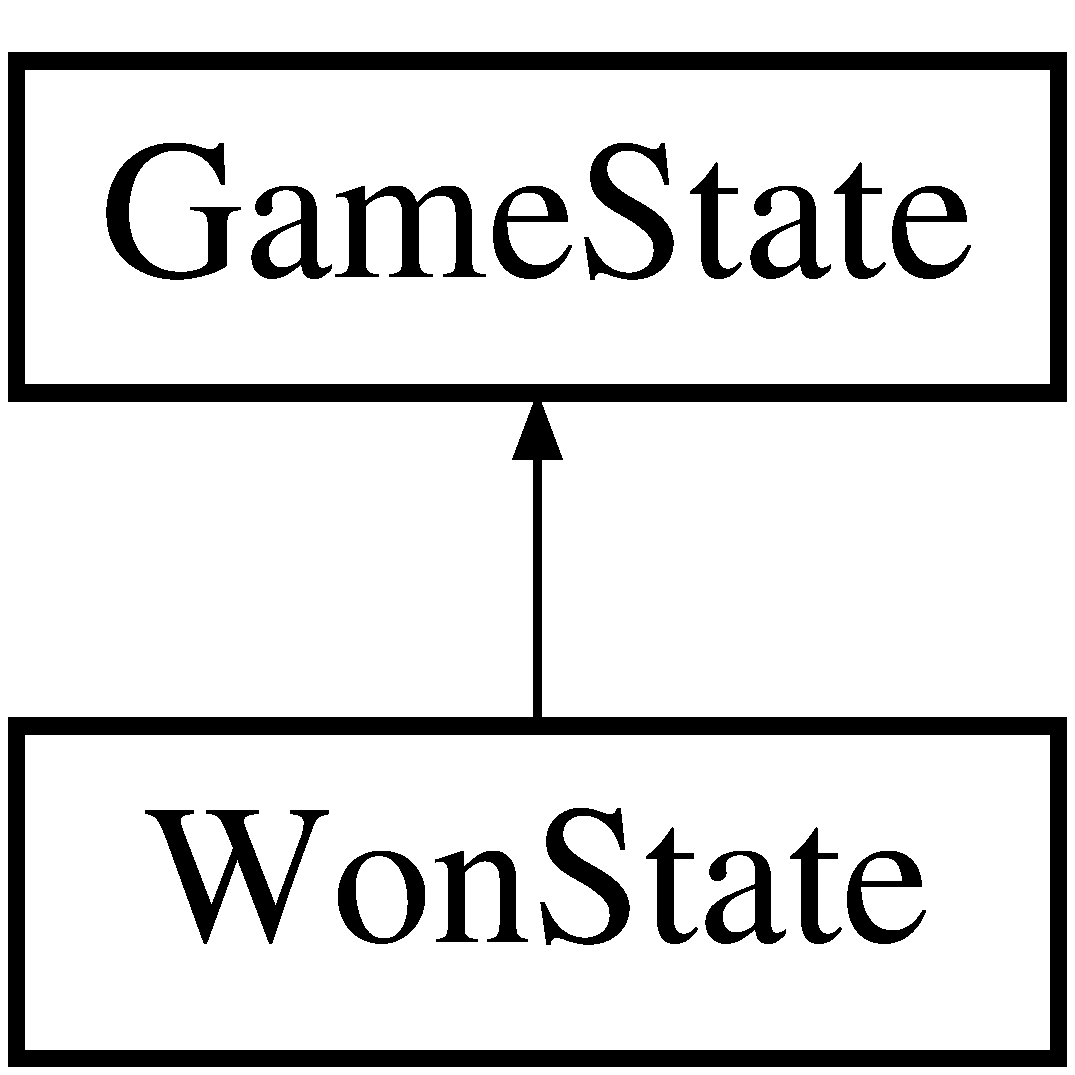
\includegraphics[height=2.000000cm]{class_won_state}
\end{center}
\end{figure}
\subsection*{Public Member Functions}
\begin{DoxyCompactItemize}
\item 
\hyperlink{class_won_state_ac6d2bf732076e157c50066c8c0331f73}{Won\+State} (\hyperlink{class_game}{Game} $\ast$a\+\_\+game, \hyperlink{class_game_state}{Game\+State} $\ast$a\+\_\+playing\+State)
\item 
void \hyperlink{class_won_state_aeaab03fa1a39188c19107047417c65b6}{insert\+Coin} ()
\item 
void \hyperlink{class_won_state_ab17f101d9ab90e60259e28b8775a76ec}{press\+Button} ()
\item 
void \hyperlink{class_won_state_a56b272d25511e6a302136d308648464b}{move\+Stick} (sf\+::\+Vector2i a\+\_\+direction)
\item 
void \hyperlink{class_won_state_a0ea91513e3df2eafbe8ef7b9810eaff1}{update} (sf\+::\+Time a\+\_\+delta)
\item 
void \hyperlink{class_won_state_a88bcef07ae234fe7ba672d1c6628d2c0}{draw} (sf\+::\+Render\+Window \&a\+\_\+window)
\end{DoxyCompactItemize}
\subsection*{Additional Inherited Members}


\subsection{Detailed Description}
\hyperlink{class_won_state}{Won\+State} Class This Class inherits from the \hyperlink{class_game_state}{Game\+State} Class. This game state announces that the play have complete the map. After 5 seconds the next game will start. 

\subsection{Constructor \& Destructor Documentation}
\mbox{\Hypertarget{class_won_state_ac6d2bf732076e157c50066c8c0331f73}\label{class_won_state_ac6d2bf732076e157c50066c8c0331f73}} 
\index{Won\+State@{Won\+State}!Won\+State@{Won\+State}}
\index{Won\+State@{Won\+State}!Won\+State@{Won\+State}}
\subsubsection{\texorpdfstring{Won\+State()}{WonState()}}
{\footnotesize\ttfamily Won\+State\+::\+Won\+State (\begin{DoxyParamCaption}\item[{\hyperlink{class_game}{Game} $\ast$}]{a\+\_\+game,  }\item[{\hyperlink{class_game_state}{Game\+State} $\ast$}]{a\+\_\+playing\+State }\end{DoxyParamCaption})}

A \hyperlink{class_won_state}{Won\+State} Constructor Intiates the text to be rendered on the screen and make sures that the scores and the number of lives are passed to the next level properly 
\begin{DoxyParams}{Parameters}
{\em a\+\_\+game} & the current game instance \\
\hline
{\em a\+\_\+playing\+State} & the current playing\+State entity \\
\hline
\end{DoxyParams}


\subsection{Member Function Documentation}
\mbox{\Hypertarget{class_won_state_a88bcef07ae234fe7ba672d1c6628d2c0}\label{class_won_state_a88bcef07ae234fe7ba672d1c6628d2c0}} 
\index{Won\+State@{Won\+State}!draw@{draw}}
\index{draw@{draw}!Won\+State@{Won\+State}}
\subsubsection{\texorpdfstring{draw()}{draw()}}
{\footnotesize\ttfamily void Won\+State\+::draw (\begin{DoxyParamCaption}\item[{sf\+::\+Render\+Window \&}]{a\+\_\+window }\end{DoxyParamCaption})\hspace{0.3cm}{\ttfamily [virtual]}}

This function renders the text to the screen


\begin{DoxyParams}{Parameters}
{\em a\+\_\+window} & the window where the game is rendered \\
\hline
\end{DoxyParams}


Implements \hyperlink{class_game_state_a5ffd5ce9acb7499ddef613e8836d1ef8}{Game\+State}.

\mbox{\Hypertarget{class_won_state_aeaab03fa1a39188c19107047417c65b6}\label{class_won_state_aeaab03fa1a39188c19107047417c65b6}} 
\index{Won\+State@{Won\+State}!insert\+Coin@{insert\+Coin}}
\index{insert\+Coin@{insert\+Coin}!Won\+State@{Won\+State}}
\subsubsection{\texorpdfstring{insert\+Coin()}{insertCoin()}}
{\footnotesize\ttfamily void Won\+State\+::insert\+Coin (\begin{DoxyParamCaption}{ }\end{DoxyParamCaption})\hspace{0.3cm}{\ttfamily [virtual]}}

This is an empty function to override it\textquotesingle{}s virtual counter part \begin{DoxySeeAlso}{See also}
\hyperlink{class_game_state}{Game\+State} Class 
\end{DoxySeeAlso}


Implements \hyperlink{class_game_state_a4cd6f5b4ad23fc08dca287df26d94b94}{Game\+State}.

\mbox{\Hypertarget{class_won_state_a56b272d25511e6a302136d308648464b}\label{class_won_state_a56b272d25511e6a302136d308648464b}} 
\index{Won\+State@{Won\+State}!move\+Stick@{move\+Stick}}
\index{move\+Stick@{move\+Stick}!Won\+State@{Won\+State}}
\subsubsection{\texorpdfstring{move\+Stick()}{moveStick()}}
{\footnotesize\ttfamily void Won\+State\+::move\+Stick (\begin{DoxyParamCaption}\item[{sf\+::\+Vector2i}]{a\+\_\+direction }\end{DoxyParamCaption})\hspace{0.3cm}{\ttfamily [virtual]}}

This is an empty function to override it\textquotesingle{}s virtual counter part \begin{DoxySeeAlso}{See also}
\hyperlink{class_game_state}{Game\+State} Class 
\end{DoxySeeAlso}

\begin{DoxyParams}{Parameters}
{\em the} & desired direction \\
\hline
\end{DoxyParams}


Implements \hyperlink{class_game_state_aaae8c1b3ae6969eb2dd81bfc12fbf43f}{Game\+State}.

\mbox{\Hypertarget{class_won_state_ab17f101d9ab90e60259e28b8775a76ec}\label{class_won_state_ab17f101d9ab90e60259e28b8775a76ec}} 
\index{Won\+State@{Won\+State}!press\+Button@{press\+Button}}
\index{press\+Button@{press\+Button}!Won\+State@{Won\+State}}
\subsubsection{\texorpdfstring{press\+Button()}{pressButton()}}
{\footnotesize\ttfamily void Won\+State\+::press\+Button (\begin{DoxyParamCaption}{ }\end{DoxyParamCaption})\hspace{0.3cm}{\ttfamily [virtual]}}

This is an empty function to override it\textquotesingle{}s virtual counter part \begin{DoxySeeAlso}{See also}
\hyperlink{class_game_state}{Game\+State} Class 
\end{DoxySeeAlso}


Implements \hyperlink{class_game_state_aa14eeaf244bcf19b7013af75cb722dde}{Game\+State}.

\mbox{\Hypertarget{class_won_state_a0ea91513e3df2eafbe8ef7b9810eaff1}\label{class_won_state_a0ea91513e3df2eafbe8ef7b9810eaff1}} 
\index{Won\+State@{Won\+State}!update@{update}}
\index{update@{update}!Won\+State@{Won\+State}}
\subsubsection{\texorpdfstring{update()}{update()}}
{\footnotesize\ttfamily void Won\+State\+::update (\begin{DoxyParamCaption}\item[{sf\+::\+Time}]{a\+\_\+delta }\end{DoxyParamCaption})\hspace{0.3cm}{\ttfamily [virtual]}}

This function switches the current game state to the get ready state to play the next level after 5 seconds. Also loads the next level before switching to the next game state.


\begin{DoxyParams}{Parameters}
{\em a\+\_\+delta} & the current time \\
\hline
\end{DoxyParams}


Implements \hyperlink{class_game_state_ab1fe4312f7ce88e7dc11f9935dee67d1}{Game\+State}.



The documentation for this class was generated from the following files\+:\begin{DoxyCompactItemize}
\item 
\hyperlink{game_state_8hpp}{game\+State.\+hpp}\item 
\hyperlink{game_state_8cpp}{game\+State.\+cpp}\end{DoxyCompactItemize}

\chapter{File Documentation}
\hypertarget{animator_8cpp}{}\section{animator.\+cpp File Reference}
\label{animator_8cpp}\index{animator.\+cpp@{animator.\+cpp}}
{\ttfamily \#include \char`\"{}animator.\+hpp\char`\"{}}\newline

\hypertarget{animator_8hpp}{}\section{animator.\+hpp File Reference}
\label{animator_8hpp}\index{animator.\+hpp@{animator.\+hpp}}
{\ttfamily \#include $<$S\+F\+M\+L/\+Graphics.\+hpp$>$}\newline
\subsection*{Classes}
\begin{DoxyCompactItemize}
\item 
class \hyperlink{class_animator}{Animator}
\end{DoxyCompactItemize}

\hypertarget{bonus_8cpp}{}\section{smfl\+Test/bonus.cpp File Reference}
\label{bonus_8cpp}\index{smfl\+Test/bonus.\+cpp@{smfl\+Test/bonus.\+cpp}}
{\ttfamily \#include \char`\"{}bonus.\+hpp\char`\"{}}\newline

\hypertarget{bonus_8hpp}{}\section{bonus.\+hpp File Reference}
\label{bonus_8hpp}\index{bonus.\+hpp@{bonus.\+hpp}}
{\ttfamily \#include $<$stdio.\+h$>$}\newline
{\ttfamily \#include \char`\"{}character.\+hpp\char`\"{}}\newline
{\ttfamily \#include $<$S\+F\+M\+L/\+Graphics.\+hpp$>$}\newline
\subsection*{Classes}
\begin{DoxyCompactItemize}
\item 
class \hyperlink{class_bonus}{Bonus}
\end{DoxyCompactItemize}

\hypertarget{character_8cpp}{}\section{character.\+cpp File Reference}
\label{character_8cpp}\index{character.\+cpp@{character.\+cpp}}
{\ttfamily \#include $<$iostream$>$}\newline
{\ttfamily \#include $<$cmath$>$}\newline
{\ttfamily \#include $<$array$>$}\newline
{\ttfamily \#include \char`\"{}character.\+hpp\char`\"{}}\newline
{\ttfamily \#include \char`\"{}define.\+h\char`\"{}}\newline

\hypertarget{character_8hpp}{}\section{smfl\+Test/character.hpp File Reference}
\label{character_8hpp}\index{smfl\+Test/character.\+hpp@{smfl\+Test/character.\+hpp}}
{\ttfamily \#include $<$S\+F\+M\+L/\+Graphics.\+hpp$>$}\newline
{\ttfamily \#include \char`\"{}maze.\+hpp\char`\"{}}\newline
\subsection*{Classes}
\begin{DoxyCompactItemize}
\item 
class \hyperlink{class_character}{Character}
\end{DoxyCompactItemize}

\hypertarget{define_8h}{}\section{smfl\+Test/define.h File Reference}
\label{define_8h}\index{smfl\+Test/define.\+h@{smfl\+Test/define.\+h}}
\subsection*{Variables}
\begin{DoxyCompactItemize}
\item 
const int \hyperlink{define_8h_aa694d481a2039c54ebfa53ea93892b0c}{S\+C\+R\+E\+E\+N\+S\+I\+Z\+E\+\_\+W} = 448
\item 
const int \hyperlink{define_8h_a556b2bf9a75429b794b0d6bfcf5bbdd1}{S\+C\+R\+E\+E\+N\+S\+I\+Z\+E\+\_\+H} = 528
\item 
const int \hyperlink{define_8h_a174e62c7a3485a80b78de97d37c78657}{C\+E\+L\+L\+S\+I\+Z\+E\+\_\+W} = 16
\item 
const int \hyperlink{define_8h_a7b3fca3c9905f883e203ae827082bfff}{C\+E\+L\+L\+S\+I\+Z\+E\+\_\+H} = 16
\end{DoxyCompactItemize}


\subsection{Variable Documentation}
\mbox{\Hypertarget{define_8h_a7b3fca3c9905f883e203ae827082bfff}\label{define_8h_a7b3fca3c9905f883e203ae827082bfff}} 
\index{define.\+h@{define.\+h}!C\+E\+L\+L\+S\+I\+Z\+E\+\_\+H@{C\+E\+L\+L\+S\+I\+Z\+E\+\_\+H}}
\index{C\+E\+L\+L\+S\+I\+Z\+E\+\_\+H@{C\+E\+L\+L\+S\+I\+Z\+E\+\_\+H}!define.\+h@{define.\+h}}
\subsubsection{\texorpdfstring{C\+E\+L\+L\+S\+I\+Z\+E\+\_\+H}{CELLSIZE\_H}}
{\footnotesize\ttfamily const int C\+E\+L\+L\+S\+I\+Z\+E\+\_\+H = 16}



Definition at line 15 of file define.\+h.

\mbox{\Hypertarget{define_8h_a174e62c7a3485a80b78de97d37c78657}\label{define_8h_a174e62c7a3485a80b78de97d37c78657}} 
\index{define.\+h@{define.\+h}!C\+E\+L\+L\+S\+I\+Z\+E\+\_\+W@{C\+E\+L\+L\+S\+I\+Z\+E\+\_\+W}}
\index{C\+E\+L\+L\+S\+I\+Z\+E\+\_\+W@{C\+E\+L\+L\+S\+I\+Z\+E\+\_\+W}!define.\+h@{define.\+h}}
\subsubsection{\texorpdfstring{C\+E\+L\+L\+S\+I\+Z\+E\+\_\+W}{CELLSIZE\_W}}
{\footnotesize\ttfamily const int C\+E\+L\+L\+S\+I\+Z\+E\+\_\+W = 16}



Definition at line 14 of file define.\+h.

\mbox{\Hypertarget{define_8h_a556b2bf9a75429b794b0d6bfcf5bbdd1}\label{define_8h_a556b2bf9a75429b794b0d6bfcf5bbdd1}} 
\index{define.\+h@{define.\+h}!S\+C\+R\+E\+E\+N\+S\+I\+Z\+E\+\_\+H@{S\+C\+R\+E\+E\+N\+S\+I\+Z\+E\+\_\+H}}
\index{S\+C\+R\+E\+E\+N\+S\+I\+Z\+E\+\_\+H@{S\+C\+R\+E\+E\+N\+S\+I\+Z\+E\+\_\+H}!define.\+h@{define.\+h}}
\subsubsection{\texorpdfstring{S\+C\+R\+E\+E\+N\+S\+I\+Z\+E\+\_\+H}{SCREENSIZE\_H}}
{\footnotesize\ttfamily const int S\+C\+R\+E\+E\+N\+S\+I\+Z\+E\+\_\+H = 528}



Definition at line 13 of file define.\+h.

\mbox{\Hypertarget{define_8h_aa694d481a2039c54ebfa53ea93892b0c}\label{define_8h_aa694d481a2039c54ebfa53ea93892b0c}} 
\index{define.\+h@{define.\+h}!S\+C\+R\+E\+E\+N\+S\+I\+Z\+E\+\_\+W@{S\+C\+R\+E\+E\+N\+S\+I\+Z\+E\+\_\+W}}
\index{S\+C\+R\+E\+E\+N\+S\+I\+Z\+E\+\_\+W@{S\+C\+R\+E\+E\+N\+S\+I\+Z\+E\+\_\+W}!define.\+h@{define.\+h}}
\subsubsection{\texorpdfstring{S\+C\+R\+E\+E\+N\+S\+I\+Z\+E\+\_\+W}{SCREENSIZE\_W}}
{\footnotesize\ttfamily const int S\+C\+R\+E\+E\+N\+S\+I\+Z\+E\+\_\+W = 448}



Definition at line 12 of file define.\+h.


\hypertarget{dot_8cpp}{}\section{dot.\+cpp File Reference}
\label{dot_8cpp}\index{dot.\+cpp@{dot.\+cpp}}
{\ttfamily \#include \char`\"{}dot.\+hpp\char`\"{}}\newline
\subsection*{Functions}
\begin{DoxyCompactItemize}
\item 
sf\+::\+Circle\+Shape \hyperlink{dot_8cpp_ac6bd5dfa751521164b1be8c7f52714b2}{get\+Dot} ()
\item 
sf\+::\+Circle\+Shape \hyperlink{dot_8cpp_a939c44faa1c7de6abcdcdc90e7265dda}{get\+Super\+Dot} ()
\end{DoxyCompactItemize}


\subsection{Function Documentation}
\mbox{\Hypertarget{dot_8cpp_ac6bd5dfa751521164b1be8c7f52714b2}\label{dot_8cpp_ac6bd5dfa751521164b1be8c7f52714b2}} 
\index{dot.\+cpp@{dot.\+cpp}!get\+Dot@{get\+Dot}}
\index{get\+Dot@{get\+Dot}!dot.\+cpp@{dot.\+cpp}}
\subsubsection{\texorpdfstring{get\+Dot()}{getDot()}}
{\footnotesize\ttfamily sf\+::\+Circle\+Shape get\+Dot (\begin{DoxyParamCaption}{ }\end{DoxyParamCaption})}

This function renders the dot for the game

\begin{DoxyReturn}{Returns}
returns the dot created 
\end{DoxyReturn}
\mbox{\Hypertarget{dot_8cpp_a939c44faa1c7de6abcdcdc90e7265dda}\label{dot_8cpp_a939c44faa1c7de6abcdcdc90e7265dda}} 
\index{dot.\+cpp@{dot.\+cpp}!get\+Super\+Dot@{get\+Super\+Dot}}
\index{get\+Super\+Dot@{get\+Super\+Dot}!dot.\+cpp@{dot.\+cpp}}
\subsubsection{\texorpdfstring{get\+Super\+Dot()}{getSuperDot()}}
{\footnotesize\ttfamily sf\+::\+Circle\+Shape get\+Super\+Dot (\begin{DoxyParamCaption}{ }\end{DoxyParamCaption})}

This function renders the super dot for the game

\begin{DoxyReturn}{Returns}
returns the super dot created 
\end{DoxyReturn}

\hypertarget{dot_8hpp}{}\section{dot.\+hpp File Reference}
\label{dot_8hpp}\index{dot.\+hpp@{dot.\+hpp}}
{\ttfamily \#include $<$S\+F\+M\+L/\+Graphics.\+hpp$>$}\newline
\subsection*{Functions}
\begin{DoxyCompactItemize}
\item 
sf\+::\+Circle\+Shape \hyperlink{dot_8hpp_ac6bd5dfa751521164b1be8c7f52714b2}{get\+Dot} ()
\item 
sf\+::\+Circle\+Shape \hyperlink{dot_8hpp_a939c44faa1c7de6abcdcdc90e7265dda}{get\+Super\+Dot} ()
\end{DoxyCompactItemize}


\subsection{Function Documentation}
\mbox{\Hypertarget{dot_8hpp_ac6bd5dfa751521164b1be8c7f52714b2}\label{dot_8hpp_ac6bd5dfa751521164b1be8c7f52714b2}} 
\index{dot.\+hpp@{dot.\+hpp}!get\+Dot@{get\+Dot}}
\index{get\+Dot@{get\+Dot}!dot.\+hpp@{dot.\+hpp}}
\subsubsection{\texorpdfstring{get\+Dot()}{getDot()}}
{\footnotesize\ttfamily sf\+::\+Circle\+Shape get\+Dot (\begin{DoxyParamCaption}{ }\end{DoxyParamCaption})}

This function renders the dot for the game

\begin{DoxyReturn}{Returns}
returns the dot created 
\end{DoxyReturn}
\mbox{\Hypertarget{dot_8hpp_a939c44faa1c7de6abcdcdc90e7265dda}\label{dot_8hpp_a939c44faa1c7de6abcdcdc90e7265dda}} 
\index{dot.\+hpp@{dot.\+hpp}!get\+Super\+Dot@{get\+Super\+Dot}}
\index{get\+Super\+Dot@{get\+Super\+Dot}!dot.\+hpp@{dot.\+hpp}}
\subsubsection{\texorpdfstring{get\+Super\+Dot()}{getSuperDot()}}
{\footnotesize\ttfamily sf\+::\+Circle\+Shape get\+Super\+Dot (\begin{DoxyParamCaption}{ }\end{DoxyParamCaption})}

This function renders the super dot for the game

\begin{DoxyReturn}{Returns}
returns the super dot created 
\end{DoxyReturn}

\hypertarget{game_8cpp}{}\section{smfl\+Test/game.cpp File Reference}
\label{game_8cpp}\index{smfl\+Test/game.\+cpp@{smfl\+Test/game.\+cpp}}
{\ttfamily \#include \char`\"{}game.\+hpp\char`\"{}}\newline
{\ttfamily \#include \char`\"{}define.\+h\char`\"{}}\newline
{\ttfamily \#include $<$iostream$>$}\newline

\hypertarget{game_8hpp}{}\section{game.\+hpp File Reference}
\label{game_8hpp}\index{game.\+hpp@{game.\+hpp}}
{\ttfamily \#include $<$iostream$>$}\newline
{\ttfamily \#include $<$S\+F\+M\+L/\+Graphics.\+hpp$>$}\newline
{\ttfamily \#include $<$array$>$}\newline
{\ttfamily \#include \char`\"{}game\+State.\+hpp\char`\"{}}\newline
\subsection*{Classes}
\begin{DoxyCompactItemize}
\item 
class \hyperlink{class_game}{Game}
\end{DoxyCompactItemize}

\hypertarget{game_state_8cpp}{}\section{smfl\+Test/game\+State.cpp File Reference}
\label{game_state_8cpp}\index{smfl\+Test/game\+State.\+cpp@{smfl\+Test/game\+State.\+cpp}}
{\ttfamily \#include \char`\"{}game\+State.\+hpp\char`\"{}}\newline
{\ttfamily \#include \char`\"{}game.\+hpp\char`\"{}}\newline
\subsection*{Functions}
\begin{DoxyCompactItemize}
\item 
{\footnotesize template$<$typename T $>$ }\\void \hyperlink{game_state_8cpp_a4ef4c9ccfb987822da7db3d431a4b272}{center\+Origin} (T \&drawable)
\end{DoxyCompactItemize}


\subsection{Function Documentation}
\mbox{\Hypertarget{game_state_8cpp_a4ef4c9ccfb987822da7db3d431a4b272}\label{game_state_8cpp_a4ef4c9ccfb987822da7db3d431a4b272}} 
\index{game\+State.\+cpp@{game\+State.\+cpp}!center\+Origin@{center\+Origin}}
\index{center\+Origin@{center\+Origin}!game\+State.\+cpp@{game\+State.\+cpp}}
\subsubsection{\texorpdfstring{center\+Origin()}{centerOrigin()}}
{\footnotesize\ttfamily template$<$typename T $>$ \\
void center\+Origin (\begin{DoxyParamCaption}\item[{T \&}]{drawable }\end{DoxyParamCaption})}



Definition at line 16 of file game\+State.\+cpp.


\hypertarget{game_state_8hpp}{}\section{smfl\+Test/game\+State.hpp File Reference}
\label{game_state_8hpp}\index{smfl\+Test/game\+State.\+hpp@{smfl\+Test/game\+State.\+hpp}}
{\ttfamily \#include $<$stdio.\+h$>$}\newline
{\ttfamily \#include $<$S\+F\+M\+L/\+Graphics.\+hpp$>$}\newline
{\ttfamily \#include \char`\"{}pacman.\+hpp\char`\"{}}\newline
{\ttfamily \#include \char`\"{}ghost.\+hpp\char`\"{}}\newline
{\ttfamily \#include \char`\"{}bonus.\+hpp\char`\"{}}\newline
{\ttfamily \#include \char`\"{}maze.\+hpp\char`\"{}}\newline
\subsection*{Classes}
\begin{DoxyCompactItemize}
\item 
class \hyperlink{class_game_state}{Game\+State}
\item 
class \hyperlink{class_no_coin_state}{No\+Coin\+State}
\item 
class \hyperlink{class_get_ready_state}{Get\+Ready\+State}
\item 
class \hyperlink{class_playing_state}{Playing\+State}
\item 
class \hyperlink{class_won_state}{Won\+State}
\item 
class \hyperlink{class_lost_state}{Lost\+State}
\end{DoxyCompactItemize}

\hypertarget{ghost_8cpp}{}\section{ghost.\+cpp File Reference}
\label{ghost_8cpp}\index{ghost.\+cpp@{ghost.\+cpp}}
{\ttfamily \#include \char`\"{}ghost.\+hpp\char`\"{}}\newline

\hypertarget{ghost_8hpp}{}\section{smfl\+Test/ghost.hpp File Reference}
\label{ghost_8hpp}\index{smfl\+Test/ghost.\+hpp@{smfl\+Test/ghost.\+hpp}}
{\ttfamily \#include $<$stdio.\+h$>$}\newline
{\ttfamily \#include $<$cmath$>$}\newline
{\ttfamily \#include \char`\"{}animator.\+hpp\char`\"{}}\newline
{\ttfamily \#include \char`\"{}character.\+hpp\char`\"{}}\newline
{\ttfamily \#include \char`\"{}pacman.\+hpp\char`\"{}}\newline
\subsection*{Classes}
\begin{DoxyCompactItemize}
\item 
class \hyperlink{class_ghost}{Ghost}
\end{DoxyCompactItemize}

\hypertarget{main_8cpp}{}\section{smfl\+Test/main.cpp File Reference}
\label{main_8cpp}\index{smfl\+Test/main.\+cpp@{smfl\+Test/main.\+cpp}}
{\ttfamily \#include $<$iostream$>$}\newline
{\ttfamily \#include \char`\"{}game.\+hpp\char`\"{}}\newline
\subsection*{Functions}
\begin{DoxyCompactItemize}
\item 
int \hyperlink{main_8cpp_a2b760810e5bb0cfb55f0c7d6d74d4438}{main} (int, char const $\ast$$\ast$)
\end{DoxyCompactItemize}


\subsection{Function Documentation}
\mbox{\Hypertarget{main_8cpp_a2b760810e5bb0cfb55f0c7d6d74d4438}\label{main_8cpp_a2b760810e5bb0cfb55f0c7d6d74d4438}} 
\index{main.\+cpp@{main.\+cpp}!main@{main}}
\index{main@{main}!main.\+cpp@{main.\+cpp}}
\subsubsection{\texorpdfstring{main()}{main()}}
{\footnotesize\ttfamily int main (\begin{DoxyParamCaption}\item[{int}]{,  }\item[{char const $\ast$$\ast$}]{ }\end{DoxyParamCaption})}

Jymar Caridad Senior Project Spring 17 

Definition at line 10 of file main.\+cpp.


\hypertarget{maze_8cpp}{}\section{maze.\+cpp File Reference}
\label{maze_8cpp}\index{maze.\+cpp@{maze.\+cpp}}
{\ttfamily \#include \char`\"{}maze.\+hpp\char`\"{}}\newline
{\ttfamily \#include \char`\"{}dot.\+hpp\char`\"{}}\newline
{\ttfamily \#include \char`\"{}bonus.\+hpp\char`\"{}}\newline
{\ttfamily \#include \char`\"{}define.\+h\char`\"{}}\newline
{\ttfamily \#include $<$iostream$>$}\newline
{\ttfamily \#include $<$cmath$>$}\newline
{\ttfamily \#include $<$cassert$>$}\newline

\hypertarget{maze_8hpp}{}\section{smfl\+Test/maze.hpp File Reference}
\label{maze_8hpp}\index{smfl\+Test/maze.\+hpp@{smfl\+Test/maze.\+hpp}}
{\ttfamily \#include $<$array$>$}\newline
{\ttfamily \#include $<$S\+F\+M\+L/\+Graphics.\+hpp$>$}\newline
\subsection*{Classes}
\begin{DoxyCompactItemize}
\item 
class \hyperlink{class_maze}{Maze}
\end{DoxyCompactItemize}

\hypertarget{pacman_8cpp}{}\section{pacman.\+cpp File Reference}
\label{pacman_8cpp}\index{pacman.\+cpp@{pacman.\+cpp}}
{\ttfamily \#include \char`\"{}pacman.\+hpp\char`\"{}}\newline

\hypertarget{pacman_8hpp}{}\section{smfl\+Test/pacman.hpp File Reference}
\label{pacman_8hpp}\index{smfl\+Test/pacman.\+hpp@{smfl\+Test/pacman.\+hpp}}
{\ttfamily \#include $<$S\+F\+M\+L/\+Graphics.\+hpp$>$}\newline
{\ttfamily \#include \char`\"{}character.\+hpp\char`\"{}}\newline
{\ttfamily \#include \char`\"{}animator.\+hpp\char`\"{}}\newline
\subsection*{Classes}
\begin{DoxyCompactItemize}
\item 
class \hyperlink{class_pacman}{Pacman}
\end{DoxyCompactItemize}

%--- End generated contents ---

% Index
\backmatter
\newpage
\phantomsection
\clearemptydoublepage
\addcontentsline{toc}{chapter}{Index}
\printindex

\end{document}
